
\chapter{The inverse ray mapping method: analytic approach}
\section{Explanation of the method}
For two-dimensional systems every ray in the PS of a line is given by a two-tuple point. Therefore, the PS of every line is a two-dimensional space.
The position coordinate in the PS of line \variabile{i} is the \variabile{x}-coordinate of the intersection point between the ray and the line \variabile{i}.
The direction coordinate is the sine of the angle that the ray forms with respect to the normal of the line \variabile{i} multiplied by the index of refraction of the medium in which the ray is located.
Let's now introduce some notation before explaining the details of the method. We indicate the PS with $\set{S}{}{}=\set{Q}{}{}\times\set{P}{}{}$,
where $\set{Q}{}{}$ is the set of the position coordinates \variabile{q} and $\set{P}{}{}$ is the set of the direction coordinates $\variabile{p}=\variabile{n}\sin{\tau}$ with $\tau$ the angle between the ray and the normal \textit{$\boldsymbol{\nu}$} of the line and \variabile{n} is the index of refraction of the medium in which the line is located.  
%The normal \vect{$\boldsymbol{\nu}$} is always directed into the cup and the angle $\tau$ between the ray and \vect{$\boldsymbol{\nu}$} is measured counterclockwise.
%In this paper we analyze only systems located in air ($\variable{n} = 1$), therefore, from now on, we do not write the index \variable{n} anymore.
%The source and the target PS of a line $\variable{i}$ are indicated with \set{S}{i}{} and \set{T}{i}{}, respectively.
%The coordinates of every ray that reaches the line $\variable{i}\in\{1, 2, 3\}$ are indicated  with $(\pos{t,}{i}, \dir{t,}{i})$ on \set{T}{i}{}.
%After reflection, the ray leaves line $\variable{i}\in\{1, 2, 3\}$ at the same position and with a new direction, the new coordinates are indicated with $(\pos{s,}{i}, \dir{s,}{i})$ on \set{S}{i}{}.
%Note that $\pos{s,}{i}= \pos{t,}{i}$ while $\dir{s,}{i}$ is obtained applying the reflection law to the direction coordinate $\dir{t,}{i}$ of the incident ray.
%The phase spaces \set{S}{i}{} and  \set{T}{i}{} of each line \variable{i} are partitioned into different regions, (\set{S}{i,}{j})$_{\variable{j}=2, 3, 4}$ and (\set{T}{i,}{k})$_{\variable{k}=1, 2, 3}$, respectively, where \variable{j}$\neq$ \variable{i} is the index of the line that is illuminated by \variable{i} and \variable{k}$\neq$ \variable{i} is the index of the line that illuminates \variable{i}. Hence, we indicate with \set{S}{i,}{j} $\subset$ \set{S}{i}{} the part of \set{S}{i}{} corresponding to rays that illuminate line \variable{j} and with \set{T}{i,}{k} $\subset$ \set{T}{i}{} the part of \set{T}{i}{} corresponding to rays originating from the line \variable{k}. Note that, due to the fact that the source only emits light, we do not define its target phase space \set{T}{$1$}{}. Similarly, since the target only receives light, its source phase space \set{S}{$4$}{} is not defined.
%For the two-faceted cup, six different phase spaces need to be considered which are given by the following expressions:
% %\begin{equation}
% %S_{\textit{i}}= \bigcup_{\begin{array}{cc}\textrm{j}=2\\\textit{j}\neq\textit{i}\end{array}}^4
% %S_{\textit{i,j}}
% %\end{equation}
%\begin{equation}
%\label{SPS}
%\begin{split}
% \mbox{\set{S}{$1$}{}} & = \mbox{\set{S}{$1$,}{$2$}}\cup
% \mbox{\set{S}{$1$,}{$3$}} \cup \mbox{\set{S}{$1$,}{$4$}},\\
%\mbox{\set{S}{$2$}{}} & =  \mbox{\set{S}{$2$,}{$3$}} \cup \mbox{\set{S}{$2$,}{$4$}},\\
%\mbox{\set{S}{$3$}{}} & =  \mbox{\set{S}{$3$,}{$2$}} \cup \mbox{\set{S}{$3$,}{$4$}},\\
%\mbox{\set{T}{$2$}{}} & = \mbox{\set{T}{$2$,}{$1$}} \cup \mbox{\set{T}{$2$,}{$3$}},\\
%\mbox{\set{T}{$3$}{}} & = \mbox{\set{T}{$3$,}{$1$}}\cup \mbox{\set{T}{$3$,}{$2$}},\\
%\mbox{\set{T}{$4$}{}} & = \mbox{\set{T}{$4$,}{$1$}}\cup \mbox{\set{T}{$4$,}{$2$}}\cup
%\mbox{\set{T}{$4$,}{$3$}}.
%\end{split}
% \end{equation}
%% \begin{equation}
%% T_{\textit{i}}= \bigcup_{\begin{array}{cc}\textrm{k}=1\\\textit{k}\neq\textit{i}\end{array}}^3 T_{\textit{i,k}}\;.
%% \end{equation}
%We need to note that, as the source cannot receive light and the target cannot emit light,  the regions $(\mbox{\set{S}{i,}{$1$}})_{\variable{i}=2,3}$ and $(\mbox{\set{T}{i,}{$4$}})_{\variable{i}=2, 3}$ are not considered.
%The boundaries $\partial \mbox{\set{S}{i,}{j}}$ are mapped into the boundaries $\partial \mbox{\set{T}{j,}{i}}$ for every $\variable{i}=\{1, 2, 3\}$ 
%and $\variable{j}=\{2, 3,4\}$ with $\variable{j}\neq \variable{i}$ (edge-ray principle \cite{Ries}). For the two-faceted cup and for all systems that are formed by straight lines, they are determined analytically (the details are explained in the next section).
%\subsection{\textbf{Computation of the boundaries of the patches with positive luminance in PS}}
%\label{sec:appendix}
% Given two lines $\variable{i}$ and $\variable{k}$
%with $\variable{i}\neq \variable{k}$, we show how to compute the boundaries of the region formed by the rays that leave line $\variable{i}$ and hit line $\variable{k}$. We do that both on \set{S}{i}{} and on \set{T}{k}{}.
%We indicate with $(\variable{x}_{\variable{i}, \ell}, \variable{z}_{\variable{i}, \ell})$ and with $(\variable{x}_{\variable{i}, \textrm{r}},\variable{z}_{\variable{i}, \textrm{r}})$ the coordinates of the points located at the left and the right extreme of line $\variable{i}$, respectively.
%Similarly, $(\variable{x}_{\variable{k}, \ell}, \variable{z}_{\variable{k}, \ell})$ and $(\variable{x}_{\variable{k}, \textrm{r}},\variable{z}_{\variable{k}, \textrm{r}})$ are the coordinates of the points located at the left and the right extreme of line $\variable{k}$, respectively.
%The boundaries $\partial$\set{S}{i,}{k} and $\partial$\set{T}{k,}{i} are obtained considering all the rays that leave the extremes of line $\variable{i}$ 
%and all the rays that reach the extremes of the target.
%Therefore, given two lines $\variable{i}$ and $\variable{k}$ with $\variable{i}\neq \variable{k}$, $\partial$\set{S}{i,}{k} and $\partial$\set{T}{k,}{i}
%are formed by four different curves,
%two of them are given by all the rays that leave the end points of line $\variable{i}$ and hit line $\variable{k}$ and, the others two are given by the rays
%that leave the extremes of line $\variable{i}$ and hit the extremes of line $\variable{k}$.
%The boundaries $\partial$\set{S}{i,}{k} and $\partial$\set{T}{k,}{i} are given by the following relations:
% \begin{equation}
%\label{eq:analytic_boundaries}
% \begin{split}
% \partial\mbox{\set{S}{i,}{k}} & = \partial\mbox{\setbound{S}{i,}{k}{\,1}}\cup \partial\mbox{\setbound{S}{i,}{k}{\,2}} \cup \partial\mbox{\setbound{S}{i,}{k}{\,3}}\cup \partial\mbox{\setbound{S}{i,}{k}{\,4}},\\
%\partial\mbox{\set{T}{k,}{i}} & = \partial\mbox{\setbound{T}{k,}{i}{\,1}}\cup \partial\mbox{\setbound{T}{k,}{i}{\,2}}\cup \partial\mbox{\setbound{T}{k,}{i}{\,3}}\cup \partial\mbox{\setbound{T}{k,}{i}{\,4}}.
% \end{split}
% \end{equation}
%$\partial$\setbound{S}{i,}{k}{1} and $\partial$\setbound{T}{k,}{i}{1} are obtained tracing out line $\variable{k}$ from
%$\variable{q}_{\variable{k}, \textrm{min}}$ to $\variable{q}_{\variable{k}, \textrm{max}}$
% by rays leaving $\variable{q}_{\variable{i}, \textrm{min}}=\variable{x}_{\variable{i}, \ell}$ with varying $\variable{p}_{\variable{i}}$, 
% $\partial$\setbound{S}{i,}{k}{1} and $\partial$\setbound{T}{k,}{i}{1} are depicted with orange lines in Figs. \ref{fig:S14} and \ref{fig:T411}, respectively;
% $\partial$\setbound{S}{i,}{k}{2} and $\partial$\setbound{T}{k,}{i}{2} are given tracing out line $\variable{i}$ from
% $\variable{q}_{\variable{i}, \textrm{min}}$ to $\variable{q}_{\variable{i}, \textrm{max}}$
% with varying $\variable{p}_{\variable{i}}$, such that all rays hit $\variable{q}_{\variable{k}, \textrm{min}}$, 
% $\partial$\setbound{S}{i,}{k}{2} and $\partial$\setbound{T}{k,}{i}{2} are depicted with green lines in Figs. \ref{fig:S14} and \ref{fig:T411}, respectively;
% $\partial$\setbound{S}{i,}{k}{3} and $\partial$\setbound{T}{k,}{i}{3} are obtained tracing out line $\variable{k}$ from
%$\variable{q}_{\variable{k}, \textrm{min}}$ to $\variable{q}_{\variable{k}, \textrm{max}}$
% by rays leaving $\variable{q}_{\variable{i}, \textrm{max}}=\variable{x}_{\variable{i}, r}$ with varying $\variable{p}_{\variable{i}}$, 
% $\partial$\setbound{S}{i,}{k}{3} and $\partial$\setbound{T}{k,}{i}{3} are depicted with red lines in Figs. \ref{fig:S14} and \ref{fig:T411}, respectively;
%  and $\partial$\setbound{S}{i,}{k}{4} and $\partial$\setbound{T}{k,}{i}{4} are given tracing out line $\variable{i}$ from
% $\variable{q}_{\variable{i}, \textrm{min}}$ to $\variable{q}_{\variable{i}, \textrm{max}}$
% with varying $\variable{p}_{\variable{i}}$, such that all rays hit $\variable{q}_{\variable{k}, \textrm{max}}$, 
% $\partial$\setbound{S}{i,}{k}{4} and $\partial$\setbound{T}{k,}{i}{4} are depicted with blue lines in Figs. \ref{fig:S14} and \ref{fig:T411}, respectively. \\ \indent
% For the two-faceted cup there is an analytic expression for the lines $\partial\mbox{\setbound{S}{i,}{k}{\variable{\,j}}}$ and
% $\partial\mbox{\setbound{T}{k,}{i}{\variable{\,j}}}$ in Eq. (\ref{eq:analytic_boundaries}) for every $\variable{j}\in\{1, \cdots, 4\}$.
% For instance, the rays on the boundaries $\partial\mbox{\setbound{S}{i,}{k}{\,1}}$ and $\partial \mbox{\setbound{T}{k,}{i}{\,1}}$
%  are parameterized in the (\variable{x}, \variable{z})-plane by the following relation:
% \begin{equation}
%\label{extremes_rays}
%\vect{r}(\variable{t})=
%\left( \begin{array}{cc}
%\variable{x}_{\variable{k}, \ell}-\variable{x}_{\variable{i}, \ell}+t(\variable{x}_{\variable{k}, \textrm{r}}-\variable{x}_{\variable{k}, \ell}) \\
%\variable{z}_{\variable{k}, \ell}-\variable{z}_{\variable{i}, \ell}+t(\variable{z}_{\variable{k}, \textrm{r}}-\variable{z}_{\variable{k},\ell})
%\end{array} \right) \qquad \quad 0\leq t\leq 1\,.
%\end{equation}
% These rays are located on a vertical line in \set{S}{i}{} as only the $\mbox{\variable{p}}_{\variable{i}}$-coordinate changes and on a curved line on \set{T}{k}{}
%  as both the target position and direction vary. The analytic expressions of $\partial \mbox{\setbound{S}{i,}{k}{\,1}}$ and $\partial \mbox{\setbound{T}{k,}{i}{\,1}}$ read:
%\begin{equation}
%\label{S_boundary}
%\partial \mbox{\setbound{S}{i,}{k}{1}}(\variable{t})=
%\left( \begin{array}{cc}
%\variable{q}_{\variable{i}, \textrm{min}} \\
%|\nu_{\variable{i}}\times \hat{\vect{r}}(\variable{t})|
%\end{array} \right),
%\end{equation}
%\begin{equation}
%\label{T_boundary}
%\partial\mbox{\setbound{T}{k,}{i}{\,1}}(\variable{t})=
%\left(\begin{array}{cc}
%\variable{q}_{\variable{i}, \textrm{max}}+t(\variable{q}_{\variable{k}, \textrm{max}}-\variable{q}_{\variable{k},\textrm{min}}) \\
%|\nu_{\variable{k}}\times \hat{\vect{r}}(\variable{t})|
%\end{array} \right)\,,
%\end{equation}
%where we have indicated with $\hat{\vect{r}}(\variable{t})$ the normalization of the ray in Eq. ($\ref{extremes_rays}$) and,
% $ \nu_\variable{i}$ and $\nu_\variable{k}$ are the normalized inward normals to lines $\variable{i}$ and $\variable{k}$, respectively.
% Note that, in order to consider the sine direction of the rays $\hat{\vect{r}}(\variable{t})$ with respect to the normal of the line that they hit,
%  we consider the modulus of the cross products $|\nu_{\variable{i}}\times \hat{\vect{r}}(\variable{t})|$ and $|\nu_{\variable{k}}\times \hat{\vect{r}}(\variable{t})|$
%  for lines $\variable{i}$ and $ \variable{k}$, respectively.
% % In Figures the boundaries $\partial$\set{S}{1}{4} and $\partial$ \set{T}{4}{1} are shown.
%  \begin{figure}
% \begin{minipage}[]{.40\textwidth}%[b]{5cm}
%   \centering
%   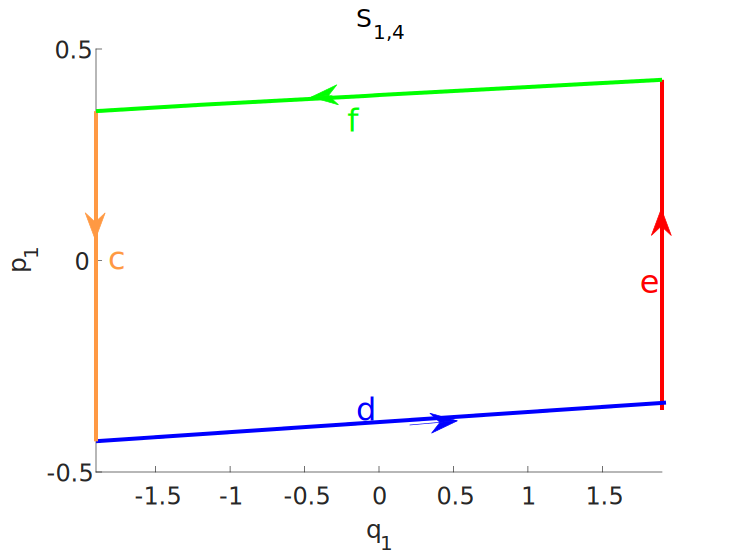
\includegraphics[width=7cm]{S141.pdf}
%   \caption{\footnotesize{Source phase space of line $1$.
%   Boundaries of the region \set{S}{$1$,}{$4$}}.}
%   \label{fig:S14}
% \end{minipage}
% \hspace{2cm}
%  \begin{minipage}[]{.40\textwidth}%[b]{5cm}
%  \centering
%   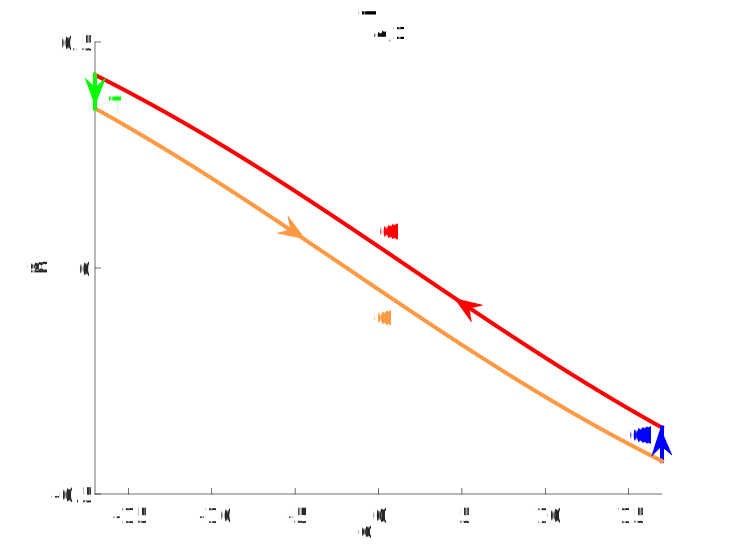
\includegraphics[width=7cm]{T411.pdf}
%   \caption{\footnotesize{Target phase space of line $4$.
%    Boundaries of the region \set{T}{$4$,}{$1$}}.}
%    \label{fig:T411}
% \end{minipage}
% \end{figure}
% Similarly, the boundaries of the lines \setbound{S}{i,}{k}{\variable{j}} and
% \setbound{T}{k,}{i}{\variable{j}} are calculated for every $\variable{j}\in\{2,3,4\}$ and
% the boundaries in Eq. (\ref{eq:analytic_boundaries}) are found. \\
% \begin{figure}
% \begin{minipage}[]{.48\textwidth}% [b]{5cm}
%  % \centering
%   \includegraphics[width=8cm]{S1.pdf}
%\caption{\footnotesize{The PS $\mbox{\set{S}{$1$}{}}$ of line $1$ is partitioned into regions $(\mbox{\set{S}{$1$,}{j}})_{\variable{j} = 2,3,4}$
%   formed by rays that leave line $1$ and hit line $\textit{j}$.}}
%   \label{fig:S1}
% \end{minipage}
%  \begin{minipage}[]{.47\textwidth}% [b]{5cm}
%  \centering
%   \includegraphics[width=8cm]{T4b.pdf}
%   \caption{\footnotesize{The PS $\mbox{\set{T}{$4$}{}}$ of line $4$ is partitioned into regions $(\mbox{\set{T}{$4$,}{k}})_{\variable{k} = 1,2,3}$
%   formed by rays that leave line $\textit{k}$ and hit line $4$.}}
%   \label{fig:T4b}
% \end{minipage}
%\begin{minipage}[]{.48\textwidth}%[b]{5cm}
%\centering
%   \includegraphics[width=8cm]{S2.pdf}
%\caption{\footnotesize{The PS $\mbox{\set{S}{$2$}{}}$ of line $2$ is partitioned into regions $(\mbox{\set{S}{$2$,}{j}})_{\variable{j} = 3,4}$,
%   formed by rays that leave line $2$ and hit line $\variable{j}$.}}
% \end{minipage}
% \begin{minipage}[]{.47\textwidth}
% \centering
%   \includegraphics[width=8cm]{T2b.pdf}
%\caption{\footnotesize{The PS $\mbox{\set{T}{$2$}{}}$ of line $2$ is partitioned into regions $(\mbox{\set{T}{$2$,}{k}})_{\variable{k} = 1,3}$
%formed by rays that leave line $\variable{k}$ and hit line $2$.}}
% \end{minipage}
% \begin{minipage}[]{.48\textwidth}
% \centering
%   \includegraphics[width=8cm]{S3.pdf}
%   \caption{\footnotesize{The PS $\mbox{\set{S}{$3$}{}}$ of line $3$ is partitioned into regions
%   $(\mbox{\set{S}{$3$,}{j}})_{\variable{j} = 2,4}$ formed by rays that leave line $3$ and hit line $\variable{j}$.}}
% \end{minipage}
% \hspace{0.8cm}
% \begin{minipage}[]{.47\textwidth}
% \centering
%   \includegraphics[width=8cm]{T3_b.pdf}
%  \caption{\footnotesize{The PS $\mbox{\set{T}{$3$}{}}$ of line $3$ is partitioned into regions $(\mbox{\set{T}{$3$,}{k}})_{\variable{k} = 1,2}$
%   formed by rays that leave line $\variable{k}$ and hit line $3$.}}
%\label{fig:T3}
% \end{minipage}
%\end{figure}
%\indent In Figs. $\ref{fig:S1}-\ref{fig:T3}$  $(\partial \mbox{\set{S}{i,}{j}})_{\variable{j}=2, 3, 4}$ and $(\partial \mbox{\set{T}{i,}{k}})_{\variable{k}=1, 2, 3}$ are depicted with blue and red lines, respectively. Indeed, those products are the sine of the angle that the ray formes with the normals $\nu_{\variable{i}}$ and $\nu_{\variable{k}}$, respectively.\\
%We observe that, because of the symmetry of the optical system, the \set{S}{$2$}{} and \set{S}{$3$}{} are symmetrical to  each other as well as \set{T}{$2$}{} and \set{T}{$3$}{}, while, due to the reflection law, \set{S}{$2$}{} and \set{T}{$2$}{} are flipped as well as \set{S}{$3$}{} and \set{T}{$3$}{}.
%In the next section, we show how the phase spaces are related to each other and we define the target photometric variables on \set{T}{$4$}{}.
%\subsection{\textbf{Target photometric variables}}
%In this section we explain how to compute the target photometric variables in PS.
%In the following, to simplify the notation, we indicate the target coordinates of the rays on \set{T}{$4$}{} with (\variable{q}, \variable{p}) instead of $(\pos{t,}{$4$}, \dir{t,}{$4$})$.
%The intensity $I$ along a given direction $\variable{p}\in [-1,1]$ in target phase space \set{T}{$4$}{} is defined as a function of the output luminance $L(\variable{q}, \variable{p})$:
%\begin{equation}\label{I(eta)}
%I_{PS}(\variable{p}) = \int_{-\variable{b}}^{\variable{b}} L(\variable{q},\variable{p}) \textrm{d}\variable{q}\,.
%\end{equation}
%Note that the intensity is a function of $\variable{p}= \sin(\theta)$ instead of $\theta$.
%The parts of \set{T}{$4$}{} that are illuminated by \set{S}{$1$}{} correspond to parts with positive luminance, for the other parts the luminance is equal to zero.
%Assuming positive luminance on \point{S}, the following relations hold:
%\begin{subequations}\label{LT4}
%\begin{align}
%L(\variable{q}, \variable{p})&>0 \qquad \quad \forall (\variable{q}, \variable{p})\in \mbox{\set{T}{$4$,}{$1$}},\\
%L(\variable{q}, \variable{p})&\geq 0 \qquad\quad \forall(\variable{q}, \variable{p}) \in (\mbox{\set{T}{$4$,}{i}})_{\variable{i}=2,3}.\label{third}
%\end{align}
%\end{subequations}
%Once a ray leaves the source \point{S} it can hit the reflectors several times before hitting the target \point{T}. To relate \point{S} and \point{T}, a map \map{M}{$1$,}{$4$}:\set{S}{$1$}{}$\rightarrow$ \set{T}{$4$}{} is introduced such that $\mbox{\map{M}{$1$,}{$4$}}(\pos{s,}{$1$},\dir{s,}{$1$})=(\variable{q},\variable{p})$.
%As  not all the parts of \set{T}{$4$}{} are illuminated by the source \point{S}, the map
%\map{M}{$1$,}{$4$} is not surjective.
%Therefore, we need to determine the subsets of \set{T}{$4$}{} illuminated by \point{S} corresponding to the regions where the luminance is positive.
%To this purpose, we consider two different kind of maps.
%The first map relates the coordinates of the source and the target PS of two \textit{different} lines, we call this map the propagation map.
%The second map relates the coordinates of the target and the source PS of the \textit{same} line, we call it the reflection map.
%In particular, given two lines \variable{i} and \variable{j} with \variable{i}$\neq$\variable{j}, the propagation map \map{P}{i,}{j}:\set{S}{i,}{j}$\mapsto$\set{T}{j,}{i} relates the regions \set{S}{i,}{j} with the regions \set{T}{j,}{i}.
%For one single line \variable{j}, the reflection map \map{R}{j}{}: \set{T}{j}{} $\mapsto$\set{S}{j}{} relates the regions \set{T}{j}{} and
%\set{S}{j,}{}. \map{P}{i,}{j} is defined as follows:
% \begin{equation}\label{Pij}
%\mbox{\map{P}{i,}{j}}(\pos{s,}{i},\dir{s,}{i})=(\pos{t,}{j},\dir{t,}{j}),
%\end{equation}
%where $\pos{t,}{j}$ is given by the \variable{x}-coordinate of the intersection point between the ray and line \variable{j},
%while $\dir{t,}{j}$ is computed considering the direction of the reflected ray with respect to the normal of line \variable{j}. \map{R}{j}{} is defined as follows:
%\begin{equation}\label{Rj}
%\mbox{\map{R}{j}{}}(\variable{q}_{\textrm{t},\textit{j}},\variable{p}_{\textrm{t},\textit{j}})=(\variable{q}_{\textrm{s},\textit{j}},\variable{p}_{\textrm{s},\textit{j}}),
%\end{equation}
% where the direction $\dir{t,}{j}$ changes according to the reflection law and the position $\pos{t,}{j}= \pos{s,}{j}$ as it maps the target PS into the source PS of the same line \variable{j}.
%Using a procedure similar to the ray transport matrices approach (see \cite{Hecht}, Chapter 6),
%the map \map{M}{$1$,}{$4$} is described by the composition of mappings \map{P}{i,}{j} and \map{R}{j}{} defined in Eqs.
%$(\ref{Pij})$ and $(\ref{Rj})$, respectively. This composition depends on the path $\Pi$ followed by the rays where we refer to a path as the sequence of lines that
% a ray hits during its propagation from \point{S} to \point{T}. We indicate with \map{M}{$1$,}{$4$}($\Pi$)
%the map \map{M}{$1$,}{$4$} restricted to path $\Pi$ and with $\mbox{\set{R}{}{}}(\Pi)\subset \mbox{\set{T}{$4$}{}}$ the regions on \set{T}{$4$}{} formed by the rays that follow path $\Pi$.
%Considering all the possible paths $\Pi$ from \point{S} to \point{T}, all the regions $\mbox{\set{R}{}{}}(\Pi)$ with positive luminance on \set{T}{$4$}{} can be determined.
%\\ \indent To clarify this concept, we provide the following example.
%Consider a ray that is emitted from the source (line $1$), hits first the left reflector (line $2$) and finally reaches the target (line $4$).
% The path $\Pi$ followed by this ray is defined as $\Pi =(1, 2, 4)$ and
% the corresponding map $\mbox{\map{M}{$1$,}{$4$}}(\Pi):\mbox{\set{S}{$1$}{}}\mapsto \mbox{\set{R}{}{}}(\Pi)$ that describes the propagation of all rays that follow the path $\Pi$ is defined by:
%\begin{equation}
%\label{map_example}
%\mbox{\map{M}{$1$,}{$4$}}(\Pi):\mbox{\set{S}{$1$,}{$2$}}\mapsto \mbox{\set{T}{$2$,}{$1$}}\mapsto\mbox{\set{S}{$2$,}{$4$}}\mapsto \mbox{\set{T}{$4$,}{$2$}}\,.
%\end{equation} Using the notation introduced above, we can write the previous relation as:
%\begin{equation}
%\mbox{\map{M}{$1$,}{$4$}}({\Pi}) = \mbox{\map{P}{$2$,}{$4$}}
%\circ \mbox{\map{R}{$2$}{}}\circ \mbox{\map{P}{$1$,}{$2$}}\,.
%\end{equation}
%Therefore, to construct the maps $\mbox{\map{M}{$1$,}{$4$}}(\Pi)$ we need to know its corresponding path $\Pi$.
%To determine all the possible paths $\Pi$,
%instead of tracing the rays from \point{S} to \point{T}, we start considering the rays in \set{T}{$4$}{}.
%In particular, along a given direction $\variable{p}\in[-1,1]$ we consider the intersection points between the line $\variable{p}=\mbox{const}$ and $(\partial\mbox{\set{T}{$4$,}{i}})_{\variable{i}\in\{1, 2, 3\}}$. These points are traced back to the line \variable{i} from which they are emitted and their corresponding coordinates on \set{S}{i}{} and \set{T}{i}{} are computed. This is done applying sequentially the maps $\mbox{\inversemap{P}{i,}{$4$}}:\mbox{\set{T}{$4$,}{i}}\mapsto\mbox{\set{S}{i,}{$4$}}$ and $\mbox{\inversemap{R}{i}{}}:\mbox{\set{S}{i}{}}\mapsto\mbox{\set{T}{i}{}}$.
%Then the same procedure is repeated considering these new coordinates on \set{T}{i}{}.
%The computation stops either when the points found are emitted from the source, that is when they are located on \set{S}{$1$}{}, or when they reach again the target, that is when they are located on \set{T}{$4$}{}.
%If the ray reaches \set{S}{$1$}{}, then a path $\Pi$ from \point{S} to \point{T} is found.
%If the ray reaches again the target \set{T}{$4$}, then we conclude that it is not emitted by
%\point{S} and therefore, it is located inside the parts of \set{T}{$4$}{} with luminance equal to zero. \\ \indent
% Finally, the inverse $\mbox{\inversemap{M}{$1$,}{$4$}}(\Pi)$ of the map \map{M}{$1$,}{$4$}$(\Pi)$ is constructed for every possible path $\Pi$.
% The map \inversemap{M}{$1$,}{$4$}$(\Pi)$ is the composition of the inverse of the propagation and the reflection maps in reverse order according to path $\Pi$.
%For instance, for path $\Pi = (1,2,4)$, \inversemap{M}{$1$,}{$4$}$(\Pi)$ is given by:
%\begin{equation}
%\label{inverse_map}
%\mbox{\inversemap{M}{$1$,}{$4$}}({\Pi}) = \mbox{\inversemap{P}{$1$,}{$2$}}
%\circ \mbox{\inversemap{R}{$2$}{}}\circ \mbox{\inversemap{P}{$2$,}{$4$}}.
%\end{equation}
%The steps of the procedure are shown in the graph in Fig. \ref{fig:tree} where the map in Eq. (\ref{inverse_map}) is written in red. \\
%\begin{figure}
%\centering
%\begin{tikzpicture}
%  [
%    grow                    = down,
%    sibling distance        = 9em,
%    level distance          = 7em,
%    edge from parent/.style = {draw, -latex},
%    selected edge from parent/.style = {draw, -latex},
%    every node/.style       = {font=\footnotesize},
%    sloped
%  ]
%  \node [root] {$\mbox{\set{T}{$4$}{}}$}
%   child { node [env] {$\mbox{\set{S}{$2$,}{$4$}}$}
%   child { node [root] {\set{T}{$2$}{}}
%   %\draw[dashed,bend right](0-1)to(0-3);
%    child { node [env] {\set{S}{$1$,}{$2$}}
%          edge from parent node [above] {\textcolor{red}{$\mathrm{P}_{1,2}^{-1}$} }}
%        child { node [env] {\set{S}{$3$,}{$2$}}
%         child { node [root] {\set{T}{$3$}{}}
%         child { node [env] {\set{S}{$1$,}{$3$}}
%             edge from parent node [above] {$\mathrm{P}_{1,3}^{-1}$}
%             }
%             child { node [env] {\set{S}{$2$,}{$3$}}
%             edge from parent node [above] {$\mathrm{P}_{2,3}^{-1}$}
%             }
%         edge from parent node [above] {$\mathrm{R}_{3}^{-1}$}
%         }
%          edge from parent node [above] {$\mathrm{P}_{3,2}^{-1}$}
%                            }
%        edge from parent node [above] {\textcolor{red}{$\mathrm{R}_{2}^{-1}$}}
%   }
%   edge from parent node [above] {\textcolor{red}{$\mathrm{P}_{2,4}^{-1}$}}
%   }
%    child { node [env] {\set{S}{$1$,}{$4$}}
%      edge from parent node [above] {$\mathrm{P}_{1,4}^{-1}$}
%      }
%    child { node [env] {\set{S}{$3$,}{$4$}}
%      child { node [root] {\set{T}{$3$}{}}
%        child { node [env] {\set{S}{$1$,}{$3$}}
%       edge from parent node [above] {$\mathrm{P}_{1,3}^{-1}$} }
%        child { node [env] {\set{S}{$2$,}{$3$}}
%         child { node [root] {\set{T}{$2$}{}}
%         child { node [env] {\set{S}{$1$,}{$2$}}
%             edge from parent node [above] {$\mathrm{P}_{1,2}^{-1}$}
%             }
%             child { node [env] {\set{S}{$3$,}{$2$}}
%             edge from parent node [above] {$\mathrm{P}_{3,2}^{-1}$}
%             }
%         edge from parent node [above] {$\mathrm{R}_{2}^{-1}$}
%         }
%          edge from parent node [above] {$\mathrm{P}_{2,3}^{-1}$}
%                           }
%            edge from parent node [above] {$\mathrm{R}_{3}^{-1}$}
%                            }
%            edge from parent node [above] {$\mathrm{P}_{3,4}^{-1}$}
%            };
%        %    \tikzset{every tree node/.style={align=center,anchor=north}}
%
%
%\end{tikzpicture}
%\\
%\caption{Tree that describes how to detect all the possible paths from \point{S} to \point{T}.}
%\label{fig:tree}
%\end{figure}
%\newpage
%\indent Using the procedure explained above, given a ray with coordinates
%$(\variable{q}, \variable{p})\in \mbox{\set{T}{$4$}{}}$ we can establish whether it is located inside one of the regions $\mbox{\set{R}{}{}}(\Pi)$ with positive luminance or not.
%In case the ray is inside a region $\mbox{\set{R}{}{}}(\Pi)$,
%its corresponding coordinates $(\pos{s,}{$1$},\dir{s,}{$1$})\in \mbox{\set{S}{$1$}{}}$ are obtained using $\mbox{\inversemap{M}{$1$,}{$4$}}(\Pi)$, where $\Pi$ is the path followed by this ray. Eq. ($\ref{LT4}$) becomes:
%\begin{subequations}\label{LT}
%\begin{align}
%L(\variable{q}, \variable{p})&>0 \qquad \quad \forall (\variable{q}, \variable{p})\in \mbox{\set{R}{}{}}(\Pi),\\
%L(\variable{q}, \variable{p})&= 0 \qquad \quad \mbox{otherwise},\label{third}
%\end{align}
%\end{subequations}
%for some path $\Pi$ connecting \point{S}{}{} and \point{T}{}{}.
%Assuming a Lambertian source and employing conservation of luminance along a ray (see \cite{Chaves}, Chapter 16), we have that $L$
%is a positive constant inside \set{R}{}{}($\Pi$) and it is equal to zero on the other parts of \set{T}{$4$}{}.
%Indicating with $\variable{q}^\textrm{\,min}(\Pi,\variable{p})$ and $\variable{q}^\textrm{\,max}(\Pi,\variable{p})$ the minimum and maximum position coordinates of the intersection points between the boundaries $ \partial$\set{R}{}{}($\Pi$) and line $\variable{p}= \mbox{const}$,
%Eq. (\ref{I(eta)}) reduces to:
%\begin{equation}\label{eta2}
%I_{PS}(\variable{p}) = \sum_{\Pi}\int_{\variable{q}^\textrm{\,min}(\Pi, \variable{p})}^{\variable{q}^\textrm{\,max}(\Pi,\variable{p})}L(\variable{q}, \variable{p})\textrm{d}\variable{q} =
%\sum_{\Pi}\big (\variable{q}^\textrm{max}(\Pi,\variable{p})-\variable{q}^\textrm{\,min}(\Pi,\variable{p})\big )\,,
%\end{equation}
%where the sum is over all the possible paths and the second equation holds as we assume $L=1$ in \set{R}{}{}($\Pi$).
%In the next paragraph the details of the procedure to compute the coordinates $\variable{q}^\textrm{\,min}(\Pi, \variable{p})$ and $\variable{q}^\textrm{\,max}(\Pi, \variable{p})$
%are explained.
%\subsection{\textbf{The structure of the algorithm}}\label{algorithm}
%The goal is to determine the intensity of the light that reaches the target in a given direction $\variable{p}=\mbox{const}$.
%Since we assume a Lambertian source, this is given by the sum of the width of the intervals formed by rays
%emitted in direction $\variable{p} = \mbox{const}$, where every interval is formed by the rays that follow the same path (see Eq. (\ref{eta2})).
%To determine these intervals, a recursive procedure is developed.
%The procedure starts considering on \set{T}{$4$}{} the two parallel rays that hit the extremes 
%of the target with direction $\variable{p}$. 
%These rays are traced back from \set{T}{$4$}{} to \set{T}{i}{} where \variable{i} is the line from which
%the traced rays are emitted. Then, another interval of parallel rays along the corresponding direction of $\variable{p} = \mbox{const}$ on \set{T}{i}{} has to be considered on \set{T}{i}{}.
%The rays corresponding
%to the points located at the extremes of this interval are traced back from $\variable{i}$ to the line from which the are emitted.
%The procedure continues recursively until the source is found.
%This allows to determine
%all the possible paths that can occur for the rays that reach the target at direction $\variable{p}$.
%Furthermore, using our method, the coordinates of the points located at the extremes of the interval formed by all the rays that follow the same path and reach the
%target at direction $\variable{p} = \mbox{const}$ can be determined.
%\\ \indent Before explaining how this can be done, let us introduce some notations.
%The coordinates on \set{T}{j}{} of points traced back from line $\variable{i}\neq\variable{j}$ to
%line $\variable{j}$ are indicated with $(\pos{t,}{j}^\textrm{\,min}, \dir{t,}{j})$ and $(\pos{t,}{j}^\textrm{\,max}, \dir{t,}{j})$ where $\pos{t,}{j}^\textrm{\,min}<\pos{t,}{j}^\textrm{\,max}$. For $\variable{j}=4$ we omit the index $\variable{j}$, so these coordinates on \set{T}{$4$}{} are indicated with
%$(\variable{q}^\textrm{\,min}, \variable{p})$ and $(\variable{q}^\textrm{\,max}, \variable{p})$ where $\variable{q}^\textrm{\,min}<\variable{q}^\textrm{\,max}$.
%The intersection points of line
%$\variable{p}= \dir{t,}{j}$ with boundaries $\partial$\set{T}{j,}{i} need to be determined for every $\variable{i} = \{1,2,3\}$ and $\variable{j} = \{2,3,4\}$ with $\variable{j}\neq\variable{i}$.
%For $\variable{j}\neq 4$, the coordinates of these intersections are indicated with $(\variable{u}_{\variable{j},\variable{i}}^\textrm{\,min}, \dir{t,}{j})$ and $(\variable{u}_{\variable{j},\variable{i}}^\textrm{\,max}, \dir{t,}{j})$ points where $\variable{u}_{\variable{j},\variable{i}}^\textrm{\,min}<\variable{u}_{\variable{j},\variable{i}}^\textrm{\,max}$.
%For $\variable{j} = 4$,
%the coordinates of the intersection points of line $\variable{p}= const$ with $\partial$\set{T}{$4$,}{i} are indicated with $(\variable{u}_{\variable{i}}^\textrm{\,min}, \variable{p})$ and $(\variable{u}_{\variable{i}}^\textrm{\,max}, \variable{p})$ for every $\variable{i}=1,2,3$.
%Since not all the rays whose corresponding coordinates are located inside the interval
%$[(\pos{t,}{j}^\textrm{\,min}, \dir{t,}{j}), (\pos{t,}{j}^\textrm{\,max}, \dir{t,}{j})]$ follow the same path,
% the intersection segment between the two intervals $[(\pos{t,}{j}^\textrm{\,min},\dir{t,}{j}),(\pos{t,}{j}^\textrm{\,max}, \dir{t,}{j})]$ and
%$[(\variable{u}_{\variable{j}, \variable{i}}^\textrm{\,min},\dir{t,}{j}) (\variable{u}_{\variable{j}, \variable{i}}^\textrm{\,max}, \dir{t,}{j})]$ need to be considered on \set{T}{j}{}.
%The coordinates of the extremes of the intersection interval
%are indicated with $(\variable{v}_{\variable{j}, \variable{i}}^\textrm{\,min},\dir{t,}{j})$ and $(\variable{v}_{\variable{j}, \variable{i}}^\textrm{\,max},\dir{t,}{j})$ where
%$\variable{v}_{\variable{j}, \variable{i}}^\textrm{\,min} = \max\{\pos{t,}{j}^ \textrm{\,min},\variable{u}_{\variable{j}, \variable{i}}^\textrm{\,min}\}$ and
% $\variable{v}_{\variable{j}, \variable{i}}^\textrm{\,max} = \min\{\pos{t,}{j}^ \textrm{\,max},\variable{u}_{\variable{j}, \variable{i}}^\textrm{\,max}\}$ when $\variable{j}\neq 4$ and with 
% $\variable{v}_{\variable{i}}^\textrm{\,min} = \max\{\pos{}{}^ \textrm{\,min},\variable{u}_{\variable{i}}^\textrm{\,min}\}$ and
% $\variable{v}_{\variable{i}}^\textrm{\,max} = \min\{\pos{}{}^ \textrm{\,max},\variable{u}_{\variable{i}}^\textrm{\,max}\}$ when $\variable{j} = 4$. \\ \indent
%To explain the technique, we make use of an example that describes how the target intensity along direction $\variable{p}= -0.2$ is calculated.
%From Fig. $\ref{fig:T41}$ to Fig. $\ref{fig:T43}$ the steps used in this example are shown.
%A detailed description of those figures is given in the following.
%\\ \indent The procedure starts considering the rays with coordinates $(\variable{q}^\textrm{min}, \variable{p})$ and $(\variable{q}^\textrm{max}, \variable{p})$ on \set{T}{$4$}{}, where $\variable{q}^\textrm{min}= -\variable{b}$ and
%$\variable{q}^\textrm{max}= \variable{b}$ are the left and the right extreme of the target \point{T}, respectively.
% The intersection points $(\variable{u}_{\variable{i}}^\textrm{\,min}, \variable{p})$ and
%$(\variable{u}_{\variable{i}}^\textrm{\,max}, \variable{p})$
%of line $\variable{p}= -0.2$
% with boundaries $\partial\mbox{\set{T}{$4$,}{i}}$ are computed for every $\variable{i}\neq 4$ (see Fig. \ref{fig:T41}). \\ \indent
%We start from boundary $\partial\mbox{\set{T}{$4$,}{$1$}}$ obtaining the rays with coordinates $(\variable{u}_{1}^\textrm{\,min}, \variable{p})$ and
%$(\variable{u}_{1}^\textrm{max}, \variable{p})$ depicted in Fig. \ref{fig:T41}.
%Then, the intersection interval $[(\variable{v}_{1}^\textrm{\,min}, \variable{p}),(\variable{v}_{1}^\textrm{\,max},\variable{p})]$ between the intervals
% $[(\variable{u}_{1}^\textrm{\,min}, \variable{p}), (\variable{u}_{1}^\textrm{\,max}, \variable{p})]$ and $[(\variable{q}^\textrm{\,min}, \variable{p}), (\variable{q}^\textrm{\,max}, \variable{p})]$ is calculated.
% Fig. \ref{fig:T41} shows that $\variable{v}_{1}^\textrm{\,max} = \variable{u}_{1}^\textrm{\,min}$ and $\variable{v}_{1}^\textrm{\,max} = \variable{u}_{1}^\textrm{\,max}$.
% As the source is reached, i.e. $\variable{i} = 1$, one possible path is found.
% The points $(\variable{v}_{1}^\textrm{\,min}, \variable{p})$
%and $(\variable{v}_{1}^\textrm{\,max}, \variable{p})$ are located on the boundaries of the region formed by the rays that leave the source and directly hit the target, that is the rays located on
%$\partial \mbox{\set{R}{}{}}(\Pi_1)$ with $\Pi_1 = (1,4)$.
%Therefore, the contribution to the intensity formed by the rays that follow the path $\Pi_1 = (1,4)$ is given by the distance between
%$(\variable{v}_{1}^\textrm{\,min}, \variable{p})$ and $(\variable{v}_{1}^\textrm{\,max}, \variable{p})$. \\ \indent
%As \set{T}{$4$}{} can be illuminated also by line $2$,
%the procedure continues considering the boundary $\partial\mbox{\set{T}{$4$,}{$2$}}$ in order to find the other paths.
%The intersection points $(\variable{u}_{2}^\textrm{\,max}, \variable{p})$ and
%$(\variable{u}_{2}^\textrm{\,max}, \variable{p})$ between line
%$\variable{p}=-0.2$ and the boundary
%$\partial\mbox{\set{T}{$4$,}{$2$}}$ are calculated.
%They are depicted in Fig. \ref{fig:T42} with the magenta dots.
%Also, $\variable{v}_{2}^\textrm{\,min} = \max\{\variable{q}^ \textrm{\,min},\variable{u}_{\variable{2}}^\textrm{\,min}\}$
%and $\variable{v}_{2}^\textrm{\,max} = \min\{\variable{q}^ \textrm{\,max},\variable{u}_{\variable{2}}^\textrm{\,max}\}$ are found.
%Their corresponding position coordinates $\pos{s,}{$2$}^\textrm{\,min}$ and $\pos{s,}{$2$}^\textrm{\,max}$ on \set{S}{$2$}{}
%are obtained using the inverse map \inversemap{P}{$2$,}{$4$}$:\mbox{\set{T}{$4$,}{$2$}}\mapsto\mbox{\set{S}{$2$,}{$4$}}$, while the directions
%$\dir{s,}{$2$}^\textrm{\,min}$ and $\dir{s,}{$2$}^\textrm{\,max} \in $\set{S}{$2$}{}
%are given considering the direction $\dir{t,}{$2$}$ with respect to the normal
%$\boldsymbol{\nu}_{2}$ of line $2$.
% Note that $\dir{s,}{$2$}^\textrm{\,min}=\dir{s,}{$2$}^\textrm{\,max}$ because lines $\variable{i}$ are straight lines and their normals $\boldsymbol{\nu}_{i}$ do not depend on the position in which it is computed.
% Then, the corresponding direction $\dir{t,}{$2$}^\textrm{\,min}=\dir{t,}{$2$}^\textrm{\,max}$ on \set{T}{$2$}{}
% is calculated employing the inverse of the reflection map \inversemap{R}{$2$}{}$:\mbox{\set{S}{$2$}{}}\mapsto \mbox{\set{T}{$2$}{}}$.
% So, applying the map $\mbox{\inversemap{R}{$2$}{}}\circ \mbox{\inversemap{P}{$4$,}{$2$}}$, depicted in red Fig. \ref{fig:tree}, to the coordinates
% $(\variable{q}^\textrm{\,min}, \variable{p})$ and
% $(\variable{q}^\textrm{\,max}, \variable{p})$, we found the points with coordinates
% $(\pos{t,}{$2$}^\textrm{\,min}, \dir{t,}{$2$})$ and
% $(\pos{t,}{$2$}^\textrm{\,max}, \dir{t,}{$2$})$ depicted in Fig. \ref{fig:T21} where $\dir{t,}{$2$}=0.82$.
% To understand whether the corresponding rays are illuminated or not by the source, the preceding procedure used for
% \set{T}{$4$}{} is now applied to \set{T}{$2$}{}
% along direction $\dir{t,}{$2$}=0.82$. \\ \indent
%  The intersection points $(\variable{u}_{2,\variable{i}}^\textrm{\,min}, \dir{t,}{$2$})$ and
%$(\variable{u}_{2,\variable{i}}^\textrm{\,max}, \dir{t,}{$2$})$
%of line $\dir{t,}{$2$}= 0.82$
% with boundaries $\partial\mbox{\set{T}{$2$,}{i}}$ are computed for every $\variable{i}\neq \{2,4\}$ (see Fig. \ref{fig:T41}).
% We start from the boundary $\partial$\set{T}{$2$,}{$1$} obtaining the points $(\variable{u}_{2, 1}^\textrm{\,min}, \dir{t,}{$2$})$ and
% $(\variable{u}_{2, 1}^\textrm{\,max}, \dir{t,}{$2$})$ shown in Fig. \ref{fig:T21}.
% Now, the position coordinates $\variable{v}_{2, 1}^\textrm{\,min} = \max\{\pos{t,}{$2$}^ \textrm{\,min},\variable{u}_{2,1}^\textrm{\,min}\}$
% and $\variable{v}_{2, 1}^\textrm{\,max} = \min\{\pos{t,}{$2$}^ \textrm{\,max},\variable{u}_{2, 1}^\textrm{\,max}\}$ need to be considered.
% All the rays located inside the segment $[(\variable{v}_{2, 1}^\textrm{\,min},\dir{t,}{$2$} ),(\variable{v}_{2, 1}^\textrm{\,max},\dir{t,}{$2$})]$
%  \set{T}{$2$}{} follow the path $\Pi_2 = (1,2,4)$. In particular, the rays corresponding to the coordinates of the
%  left and the right extreme of that segment are located on the boundaries of the region \set{R}{}{}$(\Pi_2)$ on \set{T}{$4$}{}
%  formed by all the rays that follow path $\Pi_2$.
%  Therefore, their corresponding coordinates $(\variable{q}^{\textrm{\,min}}(\Pi_2, \variable{p}), \variable{p})$ and
% $(\variable{q}^{\textrm{max}}(\Pi_2, \variable{p}), \variable{p})$ on \set{T}{$4$}{} are obtained using the direct map $\mbox{\map{P}{$4$,}{$2$}} \circ \mbox{\map{R}{2}{}}$.
%  The rays corresponding to these coordinates are located
% on the boundary $\partial$\set{R}{}{}$(\Pi_2)$ along direction $\variable{p}=-0.2$.
% The distance between them gives the contribution to the intensity $I(\variable{p})$ of the rays located in \set{R}{}{}$(\Pi_2)$ where $\variable{p}=-0.2$. \\
%\indent  \set{T}{$2$}{} can also be illuminated by line $3$, therefore the intersection points $(\variable{u}_{2, 3}^\textrm{\,max}, \dir{t,}{$2$})$
% and $(\variable{u}_{2, 3}^\textrm{\,min}, \dir{t,}{$2$})$ of line
% $\dir{t,}{$2$}=0.82$ and $\partial \mbox{\set{T}{$2$,}{$3$}}$ are calculated, these points are depicted in Fig. \ref{fig:T22}.
% The coordinates $(\variable{v}_{2, 3}^\textrm{\,min}, \dir{t,}{$2$})$ and $(\variable{v}_{2, 3}^\textrm{\,max}, \dir{t,}{$2$})$ are shown in the same figure.
% As the source is not reached yet ($\variable{i}=3$), the rays corresponding to $(\variable{v}_{2, 3}^\textrm{\,min}, \dir{t,}{$2$})$ and $(\variable{v}_{2, 3}^\textrm{\,max}, \dir{t,}{$2$})$ are followed back using the inverse of the propagation and the reflection maps.
% So first the map $\mbox{\inversemap{P}{$3$,}{$2$}}: \mbox{\set{T}{$2$,}{$3$}}\mapsto \mbox{\set{S}{$3$,}{$2$}}$
% and then the map $\mbox{\inversemap{R}{$3$}{}}: \mbox{\set{S}{$3$}{}}\mapsto \mbox{\set{T}{$3$}{}}$
% are applied to $(\variable{v}_{2, 3}^\textrm{\,min}, \dir{t,}{$2$})$ and $(\variable{v}_{2, 3}^\textrm{\,max}, \dir{t,}{$2$})$
% in order to find their coordinates
% $(\pos{t,}{$3$}^{\textrm{max}}, \dir{t,}{$3$})$ and $(\pos{t,}{$3$}^{\textrm{min}}, \dir{t,}{$3$})$ on \set{T}{$3$}{}
%with $\dir{t,}{$3$}=-0.29$. This rays are shown in Fig. \ref{fig:T31} with blue circles. \\ \indent
%The procedure continues recursively.
%  It stops either when the rays encounter the source, i.e. when $\variable{i}=1$, or when no intersection points between the
%  direction $\variable{p}=\dir{t,}{j}$ and the boundaries $\partial$\set{T}{j,}{i} are found for any $\variable{i}={1,2,3}$ with $\variable{i}\neq\variable{j}$
%  and \variable{j} the index of the target PS we are considering. \\ \indent
%  If the source is reached, then a valid path $\Pi$ is found and the corresponding coordinates $(\pos{s,}{$1$}^{\textrm{min}}, \dir{s,}{$1$})$ and
%   $(\pos{s,}{$1$}^{\textrm{max}}, \dir{s,}{$1$})$ on \set{S}{$1$}{} of the rays traced back from \point{T} to \point{S} are calculated.
%  Then, the direct map \map{M}{$1$,}{$4$}$(\Pi)$ is applied to them in order to find the coordinates $(\variable{q}^{\textrm{min}}(\Pi, \variable{p}), \variable{p})$ and
%  $(\variable{q}^{\textrm{max}}(\Pi, \variable{p}), \variable{p})$ on \set{T}{$4$}{}.
%  The contribution to the intensity due to the ray that follow the path $\Pi$ is given by the
%  distance between $(\variable{q}^{\textrm{min}}(\Pi, \variable{p}), \variable{p})$ and
%  $(\variable{q}^{\textrm{max}}(\Pi, \variable{p}), \variable{p})$. \\ \indent
%  If no intersection points are found, then the rays traced are
%  not emitted by the source, therefore no contribution to the intensity needs to be added. This is, for instance, the case of the rays with
%  coordinates $(\variable{v}_{2, 3}^\textrm{\,min}, 0.81)$ and $(\variable{v}_{2, 3}^\textrm{\,max}, 0.81)$
%  on \set{T}{$2$}{} in Fig. \ref{fig:T22}. Below we explain this case in more details. \\ \indent
%  In Fig. \ref{fig:T31}, the coordinates $(\pos{t,}{$3$}^{\textrm{max}}, \dir{t,}{$3$})$ and $(\pos{t,}{$3$}^{\textrm{min}}, \dir{t,}{$3$})$ on \set{T}{$3$}{} with $\dir{t,}{$3$}=-0.29$ are shown.
%  They are obtained applying sequentially the maps \inversemap{P}{$3,2$}{}$:\mbox{\set{T}{$2$,}{$3$}}\mapsto\mbox{\set{S}{$3$,}{$2$}}$ and \inversemap{R}{$3$}{}$:\mbox{\set{S}{$3$,}{$2$}}\subset\mbox{\set{S}{$3$}{}}\mapsto\mbox{\set{T}{$3$}{}}$ to the points $(\variable{v}_{2, 3}^\textrm{\,min}, 0.81)$ and $(\variable{v}_{2, 3}^\textrm{\,max}, 0.81)$. \\ \indent From Fig. \ref{fig:T31} we note that there are no intersection points
%   of line $\dir{t,}{$3$}=-0.29$ with $\partial\mbox{\set{T}{$3$,}{$1$}}$.
%  So, only the coordinates of the intersections $(\variable{u}_{3, 2}^\textrm{\,min}, -0.29)$ and $(\variable{u}_{3, 2}^\textrm{\,max}, -0.29)$ between line $\dir{t,}{$3$}=-0.29$ and  $\partial\mbox{\set{T}{$3$,}{$2$}}$ are calculated.
%  Next, the coordinates $(\variable{v}_{3, 2}^\textrm{\,min},-0.29)$ and $(\variable{v}_{3, 2}^\textrm{\,max}, -0.29)$ are considered.
%  Using the maps \inversemap{P}{$2,3$}{}$:\mbox{\set{T}{$3$,}{$2$}}\mapsto\mbox{\set{S}{$2$,}{$3$}}$ and
%  \inversemap{R}{$2$}{}$:\mbox{\set{S}{$2$}{}}\mapsto\mbox{\set{T}{$2$}{}}$, 
%  the corresponding coordinates $(\pos{t,}{$2$}^{\textrm{max}}, \dir{t,}{$2$})$ and $(\pos{t,}{$2$}^{\textrm{min}}, \dir{t,}{$2$})$ on \set{T}{$2$}{} are found (Fig. \ref{fig:T23})
%  with $\dir{t,}{$2$}=-0.41$.
%  Now the procedure is repeated again for \set{T}{2}{} along the direction $\dir{t,}{$2$}=-0.41$.
%  No intersection points between line $\dir{t,}{$2$}=-0.41$ and $\partial$\set{T}{$2$,}{$1$} occur.
%  Only, the intersection points $(\variable{u}_{2,3}^\textrm{\,min},\dir{t,}{$2$})$ and $(\variable{v}_{2,3}^\textrm{\,max},\dir{t,}{$2$})$
%  of line $\dir{t,}{$2$}=-0.41$ and $\partial$\set{T}{$2$,}{$3$} are found (see Fig. \ref{fig:T23}).
%  Now, the intersection interval $[(\variable{v}_{2,3}^\textrm{\,min},\dir{t,}{$2$}),(\variable{v}_{2,3}^\textrm{\,max}, \dir{t,}{$2$})]$
%between the intervals $[(\pos{t,}{$2$}^\textrm{\,min}, \dir{t,}{$2$}), (\pos{t,}{$2$}^\textrm{\,max}, \dir{t,}{$2$})]$ and
%$[(\variable{u}_{2,3}^\textrm{\,min},\dir{t,}{$2$}),(\variable{u}_{2,3}^\textrm{\,max},\dir{t,}{$2$})]$ is considered.
%Therefore, the maps \inversemap{P}{$3,2$}{}$:\mbox{\set{T}{$2$,}{$3$}}\mapsto\mbox{\set{S}{$3$,}{$2$}}$ and
%\inversemap{R}{$3$}{}$:\mbox{\set{S}{$3$}{}}\mapsto\mbox{\set{T}{$3$}{}}$ are applied to the coordinates of the extremes of
%that interval in order to find their corresponding coordinates $(\pos{t,}{$3$}^\textrm{\,min},\dir{t,}{$3$})$ and
%$(\pos{t,}{$3$}^\textrm{\,max},\dir{t,}{$3$})$
% on \set{T}{$3$}{} where $ \dir{t,}{$3$} = 0.91$ (see Fig. \ref{fig:T32}). \\ \indent
% Considering the PS \set{T}{$3$}{} and the direction $\dir{t,}{$3$}=0.91$, we note that there are no intersection points between line
% $\dir{t,}{$3$}=0.91$ and both $\partial$\set{T}{$3$,}{$1$} and $\partial$\set{T}{$3$,}{$2$}.
% Indeed, the whole segment $[(\pos{t,}{$3$}^\textrm{\,min},\dir{t,}{$3$}), (\pos{t,}{$3$}^\textrm{\,max},\dir{t,}{$3$})]$ is outside both
% \set{T}{$3$,}{$2$} and \set{T}{$3$,}{$1$}. Because of this, all the rays which corresponding coordinates inside the interval
% $[(\pos{t,}{$3$}^\textrm{\,min},\dir{t,}{$3$}), (\pos{t,}{$3$}^\textrm{\,max},\dir{t,}{$3$})]$
% are not illuminated by the source and no new real path is found. Therefore, the procedure applied to \set{T}{$2$}{$3$} stops.
%\\ \indent
%The recursive function has now to be applied to \set{T}{$4$,}{$3$}.
%The first step is depicted in Fig. \ref{fig:T43}.
% We decided to do not show all the steps for \set{T}{$4$,}{$3$} as they are similar to those used for \set{T}{$4$,}{$2$} and explained above.
% \\ \indent Finally, to compute the intensity along another direction $\variable{p}^{\variable{k}}\in[-1,1]$ on \set{T}{$4$}{},
%the procedure explained for $\variable{p}=-0.2$ is repeated for $\variable{p}= \variable{p}^{\variable{k}}$.
%In this way we find all the possible paths $\Pi$ and the regions \set{R}{}{}$(\Pi)$ with positive luminance on \set{T}{$4$}{}.
%Furthermore, considering every time the coordinates located on the boundaries of the regions \set{T}{i}{}, also the boundaries $\partial$\set{R}{}{}$(\Pi)$ are determined for a given path $\Pi$ as well as the coordinates $\variable{q}^\textrm{max}(\Pi,\variable{p})$ and $\variable{q}^\textrm{\,min}(\Pi,\variable{p})$ for every $\variable{p}\in [-1,1]$.
%In the following they are the main steps of the algorithm to calculate the intensity
%$I(\variable{p})$ along a given direction
%$\variable{p} = \variable{p}^{\variable{k}}$ in \set{T}{$4$}{}, where for the first step we take $\variable{j}=4$. \\
%\emph{\hspace*{0.5 cm} Consider the rays with coordinates $(\pos{t,}{j}^\textrm{\,min}, \dir{t,}{j})$ and
%$(\pos{t,}{j}^ \textrm{\,max},\dir{t,}{j})$ on \set{T}{j}{};
%\\ \hspace*{1cm} For every line ${\variable{i}=1,2,3} $ with $\variable{i}\neq \textrm{j}$ \\ \hspace*{2cm}
%Calculate the intersection points $(\variable{u}_{\variable{j}, \variable{i}}^\textrm{\,min}, \dir{t,}{j})$ and
%$(\variable{u}_{\variable{j}, \variable{i}}^\textrm{\,max}, \dir{t,}{j})$
%between line \\ \hspace*{2cm}  $\dir{t}{}=\dir{t,}{j}$ and
% $\partial$\set{T}{j,}{i};
% \\ \hspace*{2cm} if no intersection points are found
%\\ \hspace*{2.5cm} Stop the procedure.
%\\ \hspace*{2cm} else
%\\ \hspace*{2.5cm}
%Consider the points with coordinates $(\variable{v}_{\variable{j}, \variable{i}}^\textrm{\,min}, \dir{t,}{j})$ and
%$(\variable{v}_{\variable{j}, \variable{i}}^\textrm{\,max}, \dir{t,}{j})$
%\\ \hspace*{2.5cm} where
% $\variable{v}_{\variable{j}, \variable{i}}^\textrm{\,min}=
% \max\{\pos{t,}{j}^\textrm{\,min}, \variable{u}_{\variable{j}, \variable{i}}^\textrm{\,min}\}$, $\variable{v}_{\variable{j}, \variable{i}}^\textrm{\,max}=\min\{\pos{t,}{j}^ \textrm{\,max},\variable{u}_{\variable{j}, \variable{i}}^\textrm{\,max}\}$;
%\\ \hspace*{2.5cm}
%Apply the inverse of the propagation map \inversemap{P}{i,}{j}$:\mbox{\set{T}{j,}{i}}\mapsto\mbox{\set{T}{i,}{j}}$ to the points with coordinates
%$(\variable{v}_{\variable{j}, \variable{i}}^\textrm{\,min}, \dir{t,}{j})$ and \\
% \hspace*{2.5cm} $(\variable{v}_{\variable{j}, \variable{i}}^\textrm{\,max}, \dir{t,}{j})$ to compute their corresponding coordinates
% $(\pos{s,}{i}^\textrm{\,min}, \dir{s,}{i})$ and $(\pos{s,}{i}^\textrm{\,max},\dir{s,}{i})$ on
%\set{S}{i}{};
%\\ \hspace*{2.5cm} Apply the inverse of the reflection map
%\inversemap{R}{i}{} to the points with coordinates $(\pos{s,}{i}^\textrm{\,min},\dir{s,}{i})$ and $(\pos{s,}{i}^\textrm{\,max},\dir{s,}{i})$
% \\ \hspace*{2.5cm} on \set{S}{i}{} in order to compute their corresponding coordinates
%$(\pos{t,}{i}^\textrm{\,min}, \dir{t,}{i})$ and $(\pos{t,}{i}^\textrm{\,max}, \dir{t,}{i})$ on \set{T}{i}{};
%\\ \hspace*{2.5cm} Store the path followed by the rays traced.
%\\ \hspace*{2.5cm} if $\textit{i}=1$
%\\ \hspace*{3cm} Apply the map \map{M}{$1$,}{$4$}$(\Pi)$ to $(\pos{s,}{$1$}^\textrm{\,min},\dir{s,}{$1$})$ and
%$(\pos{s,}{$1$}^\textrm{\,max},\dir{s,}{$1$})$ on \set{S}{1}{} that have followed the path $\Pi$
%\\ \hspace*{3cm} to compute the coordinates $(\variable{q}^\textrm{\,min}(\Pi, \variable{p}),\variable{p})$ and $(\variable{q}^\textrm{\,max}(\Pi, \variable{p}),\variable{p})$
%on $\partial\mbox{\set{R}{}{}}(\Pi)$;
%\\ \hspace*{3cm} Add the contribution to the intensity using Eq. (\ref{eq:intensity});
%\\ \hspace*{3cm} Stop the procedure.
%\\ \hspace*{2.5cm} else
%\\ \hspace*{3cm} Repeat the procedure from the beginning with $\variable{j}=\variable{i}$.
%\\ \hspace*{2.5cm} end
%\\ \hspace*{2cm} end
%\\ \hspace*{1cm} end
%} \\
%
%\begin{figure}
%\begin{minipage}[b]{15 cm}
%\centering
%   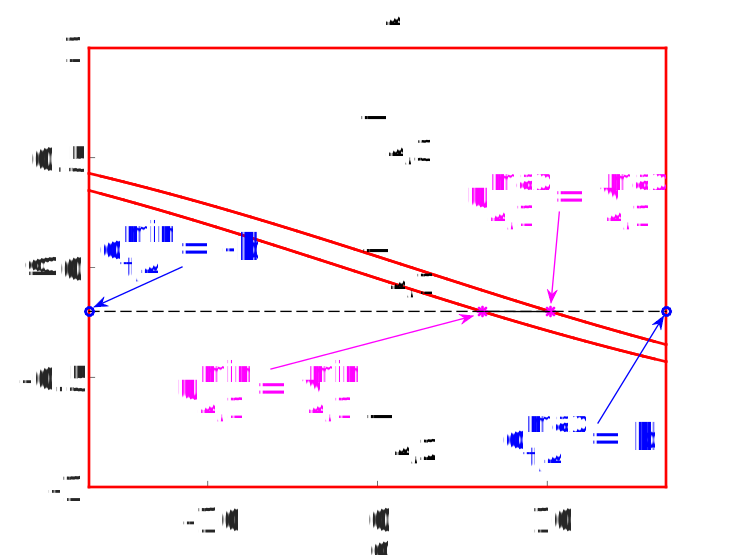
\includegraphics[width=6.7cm]{T4_1.pdf}
%  \caption{\footnotesize{Target phase space of line $4$. $\variable{q}^{\textrm{min}}$ and $\variable{q}^{\textrm{max}}$ are the $\variable{x}$-coordinates of extremes of line $4$.
%  The intersection points between the line $\variable{p} = -0.2$ and $\partial$\set{T}{$4$,}{$1$} are $(\variable{u}_{1}^{\textrm{min}}, \variable{p})$ and
%  $(\variable{u}_{1}^{\textrm{max}}, \variable{p})$. $\variable{v}_{1}^{\textrm{min}}= \max \{\variable{q}^{\textrm{min}}, \variable{u}_{1}^{\textrm{min}}\}$ and
%  $\variable{v}_{1}^{\textrm{max}}= \min \{\variable{q}^{\textrm{max}}, \variable{u}_{1}^{\textrm{max}}\}$.
%   The intensity related to the rays that follow the path
%  $\Pi =(1,4)$ is given by $|\variable{v}_{1}^{\textrm{min}}-\variable{v}_{1}^{\textrm{max}}|$ .}}
%   \label{fig:T41}
%\end{minipage}
% \begin{minipage}[]{.40\textwidth}
%  \centering
%   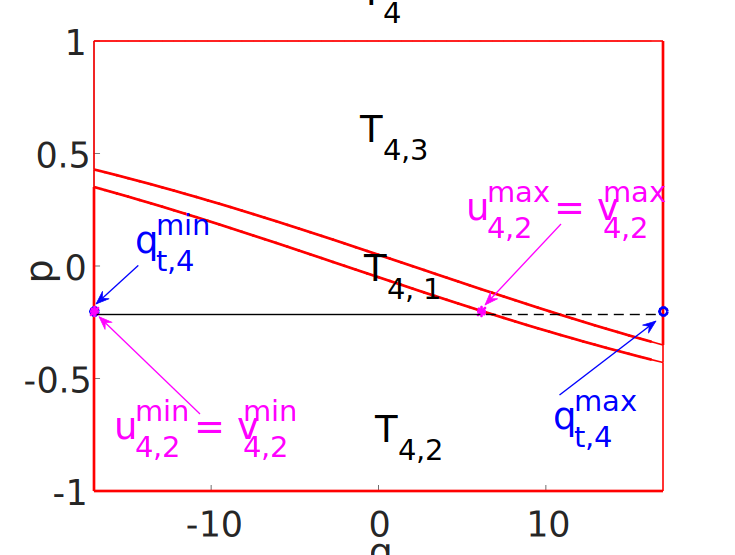
\includegraphics[width=6.7cm]{T4_2.pdf}
%   \caption{\footnotesize{Target phase space of line $4$. The coordinates $\variable{q}^{\textrm{min}}$ and $\variable{q}^{\textrm{max}}$
%   are the $\variable{x}$-coordinates of extremes of line $4$.
%  The intersection points between the line $\variable{p} = -0.2$ and $\partial$\set{T}{$4$,}{$2$} are $(\variable{u}_{2}^{\textrm{min}}, \variable{p})$ and
%  $(\variable{u}_{2}^{\textrm{max}}, \variable{p})$. $\variable{v}_{2}^{\textrm{min}}= \max \{\variable{q}^{\textrm{min}}, \variable{u}_{2}^{\textrm{min}}\}$ and
%  $\variable{v}_{2}^{\textrm{max}}= \min \{\variable{q}^{\textrm{max}}, \variable{u}_{2}^{\textrm{max}}\}$.}}
%   \label{fig:T42}
% \end{minipage}
% \begin{minipage}[]{.40\textwidth}
%   \centering
%   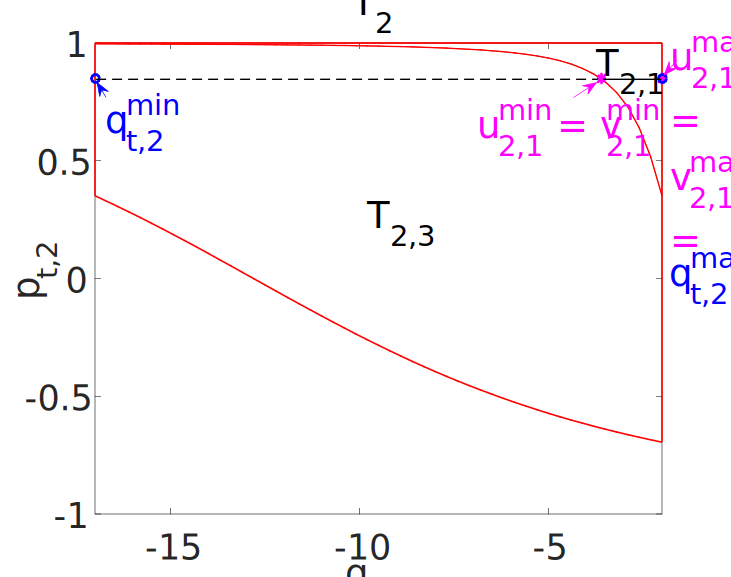
\includegraphics[width=6.7cm]{T2_1.pdf}
%   \caption{\footnotesize{Target phase space of line $2$. The coordinates
%   $(\pos{t,}{$2$}^{\textrm{min}}, 0.82)$ and $(\pos{t,}{$2$}^{\textrm{max}}, 0.82)$ are obtained applying the map $\mbox{\inversemap{R}{$2$}{}}\circ\mbox{\inversemap{P}{$2$,}{$4$}}$ to the points $(\variable{v}_{2}^{\textrm{min}},\variable{p})$ and $(\variable{v}_{2}^{\textrm{max}}, \variable{p})$, respectively. The coordinates of the intersection points between line $\dir{t,}{$2$} = 0.82$ and $\partial$\set{T}{$2$,}{$1$} are
%  $(\variable{u}_{2,1}^{\textrm{min}}, \variable{p})$ and $(\variable{u}_{2,1}^{\textrm{max}}, \variable{p}$).\\
%  $\variable{v}_{2,1}^{\textrm{min}}= \max \{\pos{t,}{$2$}^{\textrm{min}}, \variable{u}_{2,1}^{\textrm{min}}\}$ and
%  $\variable{v}_{2,1}^{\textrm{max}}= \min \{\pos{t,}{$2$}^{\textrm{max}}, \variable{u}_{2,1}^{\textrm{max}}\}$.
% }}
%    \label{fig:T21}
% \end{minipage}
% \begin{minipage}[]{.40\textwidth}
%  \centering
%   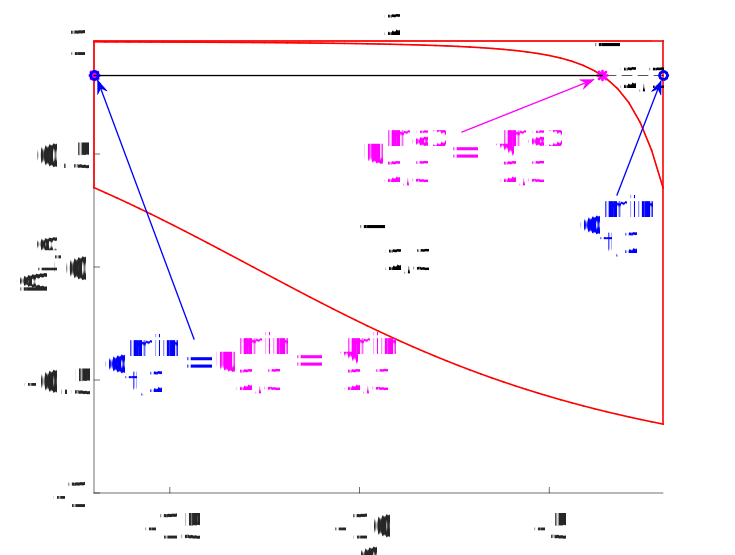
\includegraphics[width=6.7cm]{T2_2.pdf}
%\caption{\footnotesize{Target phase space of line $2$.
%The coordinates $(\pos{t,}{$2$}^{\textrm{min}}, 0.82)$ and $(\pos{t,}{$2$}^{\textrm{max}}, 0.82)$ are obtained applying the map $\mbox{\inversemap{R}{$2$}{}}\circ\mbox{\inversemap{P}{$2$,}{$4$}}$ to the points $(\variable{v}_{2}^{\textrm{min}},\variable{p})$ and
%$(\variable{v}_{2}^{\textrm{max}}, \variable{p})$, respectively.
%  The coordinates of the intersection points between line $\dir{t,}{$2$}=0.82$ and $\partial$\set{T}{$2$,}{$3$} are
%  $(\variable{u}_{2,3}^{\textrm{min}}, 0.82)$ and $(\variable{u}_{2,3}^{\textrm{max}}, 0.82)$.
%  $\variable{v}_{2,3 }^{\textrm{min}} = \max\{\variable{u}_{2,3}^{\textrm{min}}, \pos{t,}{$2$}^{\textrm{min}}\}$ and
%   $\variable{v}_{2,3 }^{\textrm{max}} = \min\{\variable{u}_{2,3}^{\textrm{max}}, \pos{t,}{$3$}^{\textrm{max}}\}$.
%}} \label{fig:T22}
% \end{minipage}
% \hspace{3cm}
%  \begin{minipage}[]{.40\textwidth}
%   \centering
%   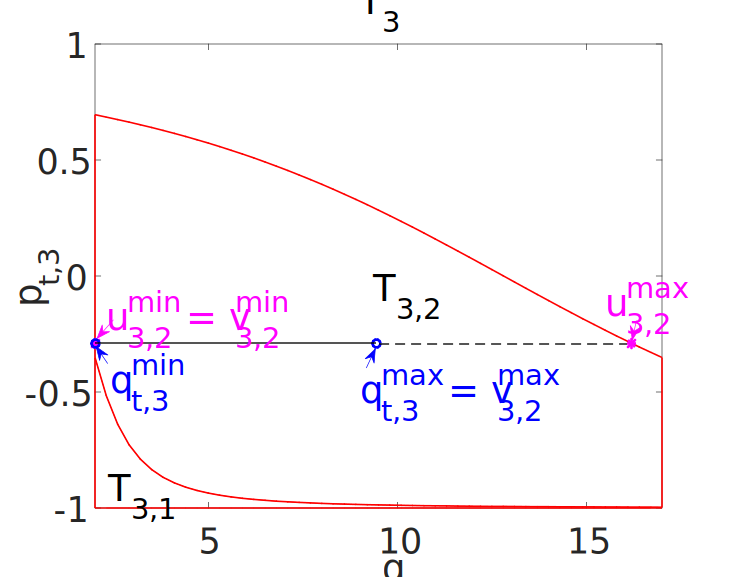
\includegraphics[width=6.7cm]{T3_1.pdf}
%   \caption{\footnotesize{Target phase space of line $3$.
%   The coordinates $(\pos{t,}{$3$}^{\textrm{min}}, -0.29)$ and $(\pos{t,}{$3$}^{\textrm{max}},-0.29 )$ are obtained applying the map
%   $\mbox{\inversemap{R}{$3$}{}}\circ\mbox{\inversemap{P}{$3$,}{$2$}}$ to the points
%   $(\variable{v}_{2,3}^{\textrm{min}}, \dir{t,}{$2$})$ and $(\variable{v}_{2,3}^{\textrm{max}}, \dir{t,}{$2$})$.
%  The position coordinates of the intersection points between line line $ \dir{t,}{$3$} = -0.29$ and
%  $\partial$\set{T}{$3$,}{$2$} are $\variable{u}_{3,2}^{\textrm{min}}$ and $\variable{u}_{3,2}^{\textrm{max}}$.
%   $\variable{v}_{3,2 }^{\textrm{min}} = \max\{\variable{u}_{3,2}^{\textrm{min}}, \pos{t,}{$3$}^{\textrm{min}}\}$ and
%   $\variable{v}_{3,2 }^{\textrm{max}} = \min\{\variable{u}_{3,2}^{\textrm{max}}, \pos{t,}{$3$}^{\textrm{max}}\}$.}}
%   \label{fig:T31}
% \end{minipage}
% \end{figure}
% \begin{figure}
% \begin{minipage}[]{.40\textwidth}
%  \centering
%   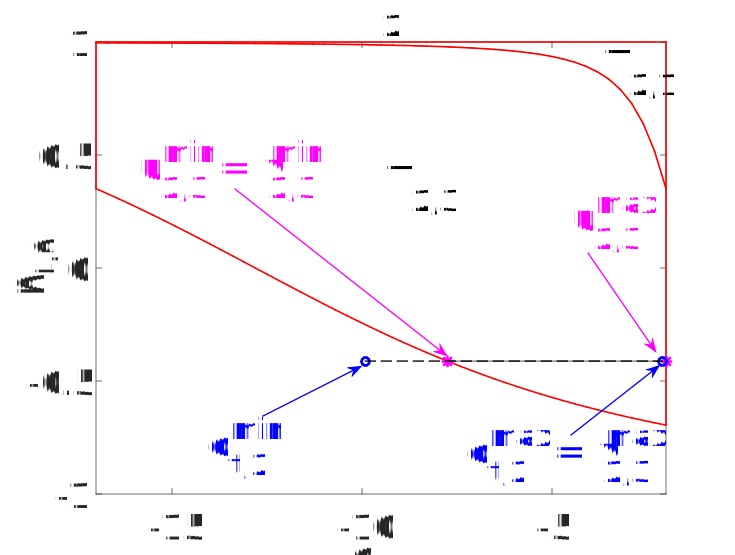
\includegraphics[width=6.7cm]{T2_3.pdf}
% \caption{\footnotesize{Target phase phase of line $2$. The coordinates of the points $(\pos{t,}{$2$}^{\textrm{min}}, -0.41)$
% and $(\pos{t,}{$2$}^{\textrm{max}},-0.41 )$ are obtained applying the map $\mbox{\inversemap{R}{$2$}{}}\circ\mbox{\inversemap{P}{$2$,}{$3$}}$
% to the points
% $(\variable{v}_{3,2 }^{\textrm{min}}, -0.29)$ and $(\variable{v}_{3,2 }^{\textrm{max}},-0.29 )$.
% The intersection points between line $\dir{t}{} = \dir{t,}{$2$}$ and $\partial$\set{T}{$2$,}{$3$} are
% $(\variable{u}_{2,3}^{\textrm{min}}, \dir{t,}{$2$})$ and $(\variable{u}_{2,3}^{\textrm{max}}, \dir{t,}{$2$})$.
% $\variable{v}_{2,3 }^{\textrm{min}} = \max\{\variable{u}_{2,3}^{\textrm{min}}, \pos{t,}{$2$}^{\textrm{min}}\}$ and
% $\variable{v}_{2,3 }^{\textrm{max}} = \min\{\variable{u}_{2,3}^{\textrm{max}}, \pos{t,}{$2$}^{\textrm{max}}\}$.}}
%    \label{fig:T23}
% \end{minipage}
% \hspace{2mm}
%  \begin{minipage}[]{.40\textwidth}
%   \centering
%   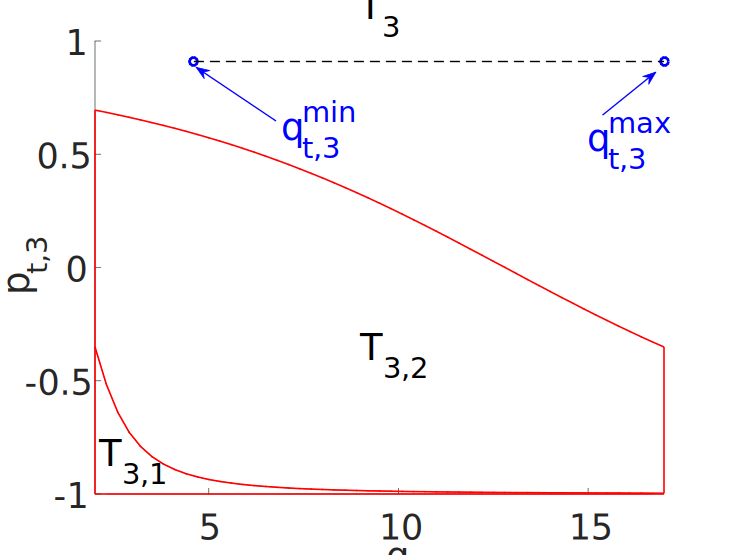
\includegraphics[width=6.7cm]{T3_2.pdf}
%   \caption{\footnotesize{Target phase space of line $3$. The coordinates of the points $(\pos{t,}{$3$}^{\textrm{min}}, 0.91)$ and
%   $(\pos{t,}{$3$}^{\textrm{max}}, 0.91)$ are obtained applying the map $\mbox{\inversemap{R}{$3$}{}}\circ\mbox{\inversemap{P}{$3$,}{$2$}}$ to the points
% $(\variable{v}_{3,2}^{\textrm{min}}, -0.29)$ and $(\variable{v}_{3,2}^{\textrm{max}},-0.29 )$.
%  There are no intersection points of line $\dir{$3$,}{$2$}=0.91$
% with the boundaries $\partial$\set{T}{$3$,}{$2$} and $\partial$\set{T}{$3$,}{$1$}.
%  The rays with coordinates equal to the coordinates of the extremes of the dotted segment hit again line $4$ after some reflection inside the system.
%   These rays are not emitted from the source.}}
%    \label{fig:T32}
% \end{minipage}
% \begin{minipage}[b]{15 cm}
%   \centering
%   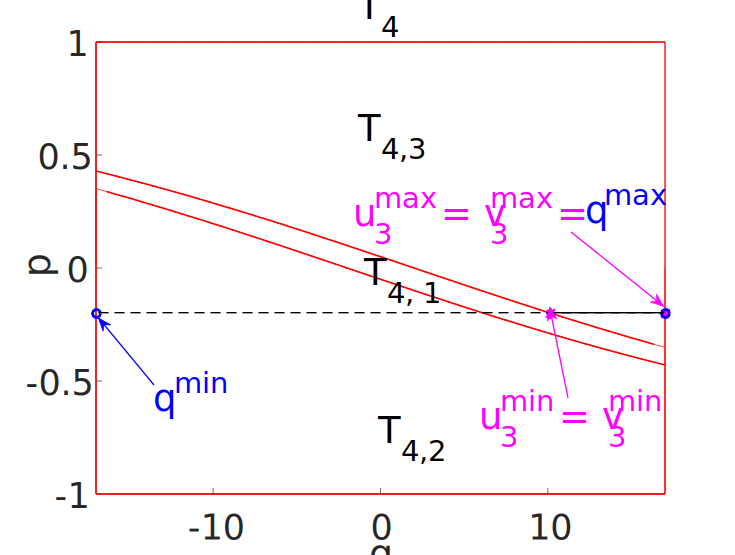
\includegraphics[width=6.7cm]{T4_3.pdf}
%   \caption{\footnotesize{Target phase space of line $4$. The rays depicted with the blue circles have as position coordinates the coordinates of the extremes of the target.
%  The intersection points between line $\variable{p} = -0.2$ and $\partial$\set{T}{$4$,}{$3$} are $(\variable{u}_{3}^{\textrm{min}}, \variable{p})$ and $(\variable{u}_{4,3}^{\textrm{max}}, \variable{p})$. $\variable{v}_{3}^{\textrm{min}} = \max\{\variable{u}_{3}^{\textrm{min}}, \pos{t,}{$3$}^{\textrm{min}}\}$
%  and $\variable{v}_{3}^{\textrm{max}} = \min\{\variable{u}_{3}^{\textrm{max}}, \pos{t,}{$3$}^{\textrm{max}}\}$.
%  The same procedure applied for the region \set{T}{$4$,}{$2$} is repeated for the region \set{T}{$4$,}{$3$}}}
%   \label{fig:T43}
%\end{minipage}
%\end{figure}
% \indent In the next section we provide the numerical results for the two-faceted cup. \newpage
% \section{Numerical results for the two-faceted cup}
%\label{sec:Numerical results_cup}
%%In this section we show a comparison between the MC intensity with the intensity found with our method.
%To demonstrate the accuracy of the method, a comparison with the ray tracing approach is provided.
%In particular, we compare our method with MC ray tracing.
%The MC intensity is computed tracing randomly a large number of rays from the source to the target of the system.
%Then, a partitioning $P:-1\leq \variable{p}^1 < \cdots< \variable{p}^\textrm{Nb} \leq 1$ of the interval $[-1,1]$ is considered and the number of rays that fall into each bin $[\variable{p}^\variable{h}, \variable{p}^{\variable{h}+1}]_{\variable{h} = 1, \cdots,\textrm{Nb}-1}$ (subintervals of the same length) is calculated for all $\variable{h} \in\{1, \cdots, \variable{Nb}-1\}$.
%The averaged and normalized MC intensity along the direction $\variable{p}^{\variable{h}+1/2}\in[\variable{p}^\variable{h}, \variable{p}^{\variable{h}+1}]$ is given by:
% \begin{equation}\label{eq:MC_intensity}
% \hat{I}_{\textrm{MC}}(\variable{p}^{\variable{h}+1/2}) = \frac{\textrm{Nr}[\variable{p}^\variable{h}, \variable{p}^{\variable{h}+1}]}{\textrm{Nr}[-1, 1]}, \end{equation}
% for every $\Big(\variable{p}^{\variable{h}+1/2} = \frac{1}{2}(\variable{p}^{\variable{h}+1}+\variable{p}^\variable{h})\Big)_{\variable{h} = 1, \cdots, \textrm{Nb}-1}$, where we have indicated with $\textrm{Nr}[\variable{p}^\variable{h}, \variable{p}^{\variable{h}+1}]$ the number of rays that fall into the bin $[\variable{p}^\variable{h}, \variable{p}^{\variable{h}+1}]$ and with $\textrm{Nr}[-1, 1]$ the number of rays that reach the target. Hence, the MC intensity is a piecewise constant intensity where the value of the constant along a given direction is obtained by the average of the intensity over the bin.\\
%\indent In order to compute the intensity distribution along all the directions, the partitioning $P$ of the target is considered. Then, the procedure explained above is repeated for $\variable{p} = (\variable{p}^\variable{h})_{\variable{h}=1, \cdots, \textrm{Nb}}$ and the averaged intensity is calculated over every bin.\\
%The averaged normalized intensity in PS is given by:
%\begin{equation}\label{eq:intensity}
% \hat{I}_{\textrm{PS}}(\variable{p}^{\variable{h}+1/2}) = \frac{\int_{\variable{p}^\variable{h}}^{\variable{p}^{\variable{h}+1}}{I}_{PS}(\variable{p})\textrm{d}\variable{p}}{\int_{-1}^{1}{I}_{PS}(\variable{p})\textrm{d}\variable{p}} \quad \mbox{for} \quad \variable{h} = 1,2, \cdots, \textrm{Nb}-1\,,
% \end{equation}
% where the integrals in the previous equation are calculated using the trapezoidal method.\\
%The accuracy of the methods is obtained by the calculation of the error between the approximated intensities
%and a reference intensity.
%For the two-faceted cup the intensity can be computed analytically.
%This intensity is taken as a reference intensity.
%Defining the partitioning $P = -1\leq \variable{p}^{1}< \cdots<\variable{p}^\textrm{Nb}\leq 1$ at the target with $\textrm{Nb}=100$, Eq. ($\ref{eq:MC_intensity}$) is used to calculate the target intensity with the MC ray tracing method tracing $10^7$ rays.
%The MC intensity is depicted in Fig. \ref{fig:intensity_cup} with a blue line.
%Then, we compute the intensity at the target employing the phase space method. Using the procedure explained in Section \ref{sec:Phase space} we are able to detect all the possible paths $\Pi$ that a ray can follow during the propagation through the system. Furthermore, given a path $\Pi$, the coordinates $(\variable{q}^\textrm{min}(\Pi, \variable{p}^ \variable{h}), \variable{p}^ \variable{h})$ and $(\variable{q}^\textrm{\,max}(\Pi, \variable{p}^ \variable{h}), \variable{p}^\variable{h})$ of the rays located on $\partial \mbox{\set{R}{}{}}(\Pi)$ are determined for every $\variable{p}^\variable{h}$ in the same partitioning $P$ used for MC ray tracing.
%These rays are depicted with blue dots in Fig. \ref{fig:final_T}.
%Note from Fig.$\ref{fig:final_T}$ that only $200$ rays need to be traced through the system for the intensity computation.
%\begin{figure}[h]
%  \begin{center}
%  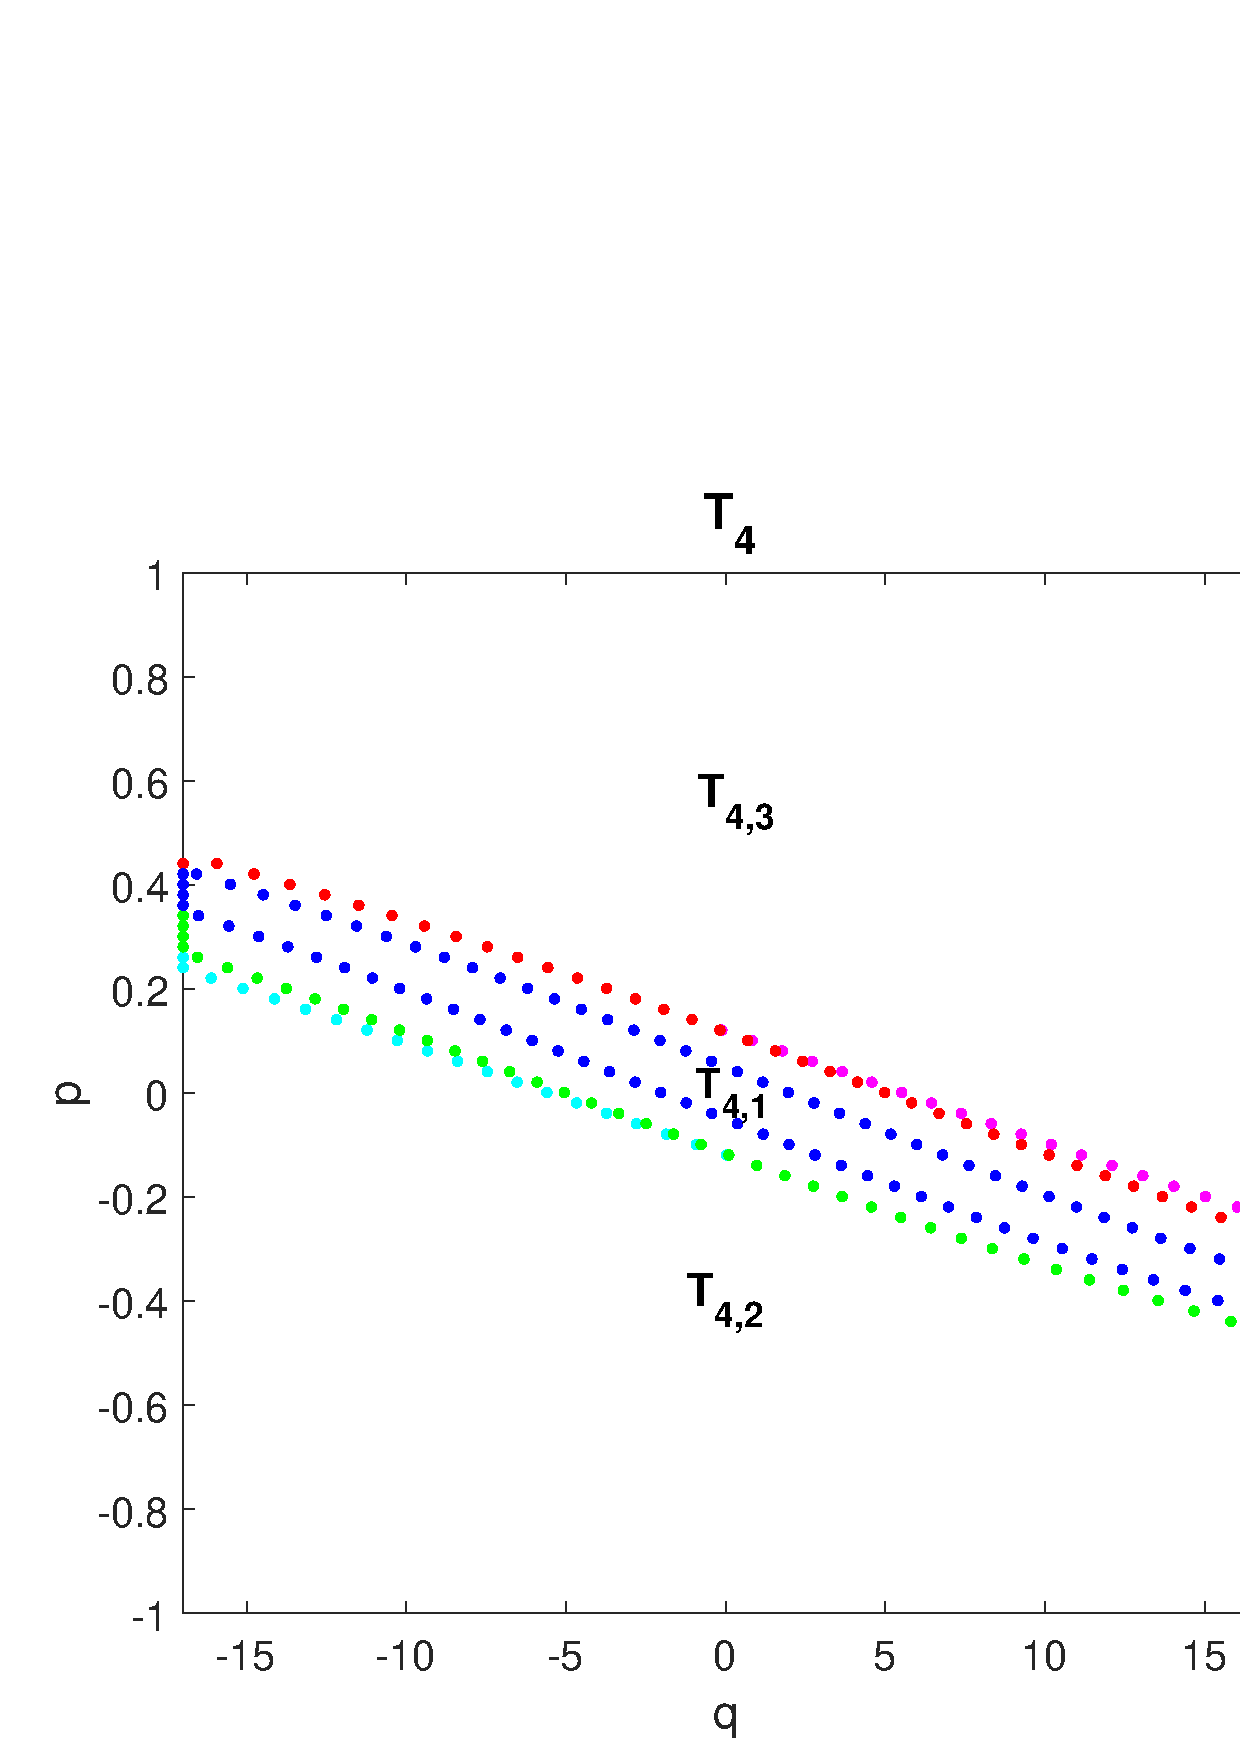
\includegraphics[scale=.4]{final_T.pdf}
%  \end{center}
%  \caption{\footnotesize{Target phase space for the two-faceted cup.
%  Five different paths are found. The rays with coordinates $(\variable{q}^\textrm{\,min}, \variable{p})$ and $(\variable{q}^\textrm{\,max}, \variable{p})$ in \set{T}{$4$}{} that are located at the boundaries $\partial \mbox{\set{R}{}{}}(\Pi)$ are depicted with dots, the color of the dots depends on the path $\Pi$ followed by the rays.
%  Using the ray mapping method, only these rays need to be traced from $\point{S}$ to $\point{T}$ for the intensity computation.}}
%  \label{fig:final_T}
%\end{figure} \\
%Finally, the phase space intensity $\hat{I}_{\textrm{PS}}$ is computed using Eq. (\ref{eq:intensity}).
%The profile of the PS intensity is depicted in in Fig. \ref{fig:intensity_cup} with the dotted green line.
%The results in Fig. \ref{fig:intensity_cup} show that all the intensity's profiles are similar. Therefore, we can claim that our method computes the intensity correctly. Moreover, the accuracy of the intensity does not depends on the number of rays traced. \\ \indent
%In order to compare the speed of convergence of the two methods, we consider the error between the approximate intensities $\hat{I}_{\textrm{A}}$ ($\textrm{A} = \textrm{MC}, \textrm{PS}$) and the reference intensity $\hat{I}_{\mbox{ref}}$. This error is defined as:
%\begin{equation}\label{error}
%\mbox{error} = \frac{\sum_{\variable{h} = 1}^{\textrm{Nb}}| \hat{I}_{\textrm{A}}(\variable{p}^\variable{h}) - \hat{I}_{\textrm{ref}}(\variable{p}^\variable{h})|}{\textrm{Nb}}\,.
%\end{equation}
%As the accuracy of the ray tracing method depends on the number of rays traced, the MC intensity is calculated for increasing number of rays traced through the system and, the error between the approximate intensity and the reference intensity is computed using Eq. (\ref{error}). In Fig. $\ref{fig:error_cup}$ the behavior of the MC error as a function of the CPU-time is depicted with the blue line. Increasing the number of rays the MC error decreases proportionally to the inverse of the square root of the number of rays traced. Then, the PS error is computed using Eq. (\ref{error}). It is depicted in Fig. $\ref{fig:error_cup}$ with the green dot. From the numerical results shown in Fig. $\ref{fig:error_cup}$ we can conclude that the PS ray mapping method is able to compute the output intensity of the two-faceted cup analytically.
%In addiction, it is faster than the classical ray tracing approach when an error smaller than $10^
%{-4}$ is required.
%\begin{figure}[h]
%  \begin{center}
%  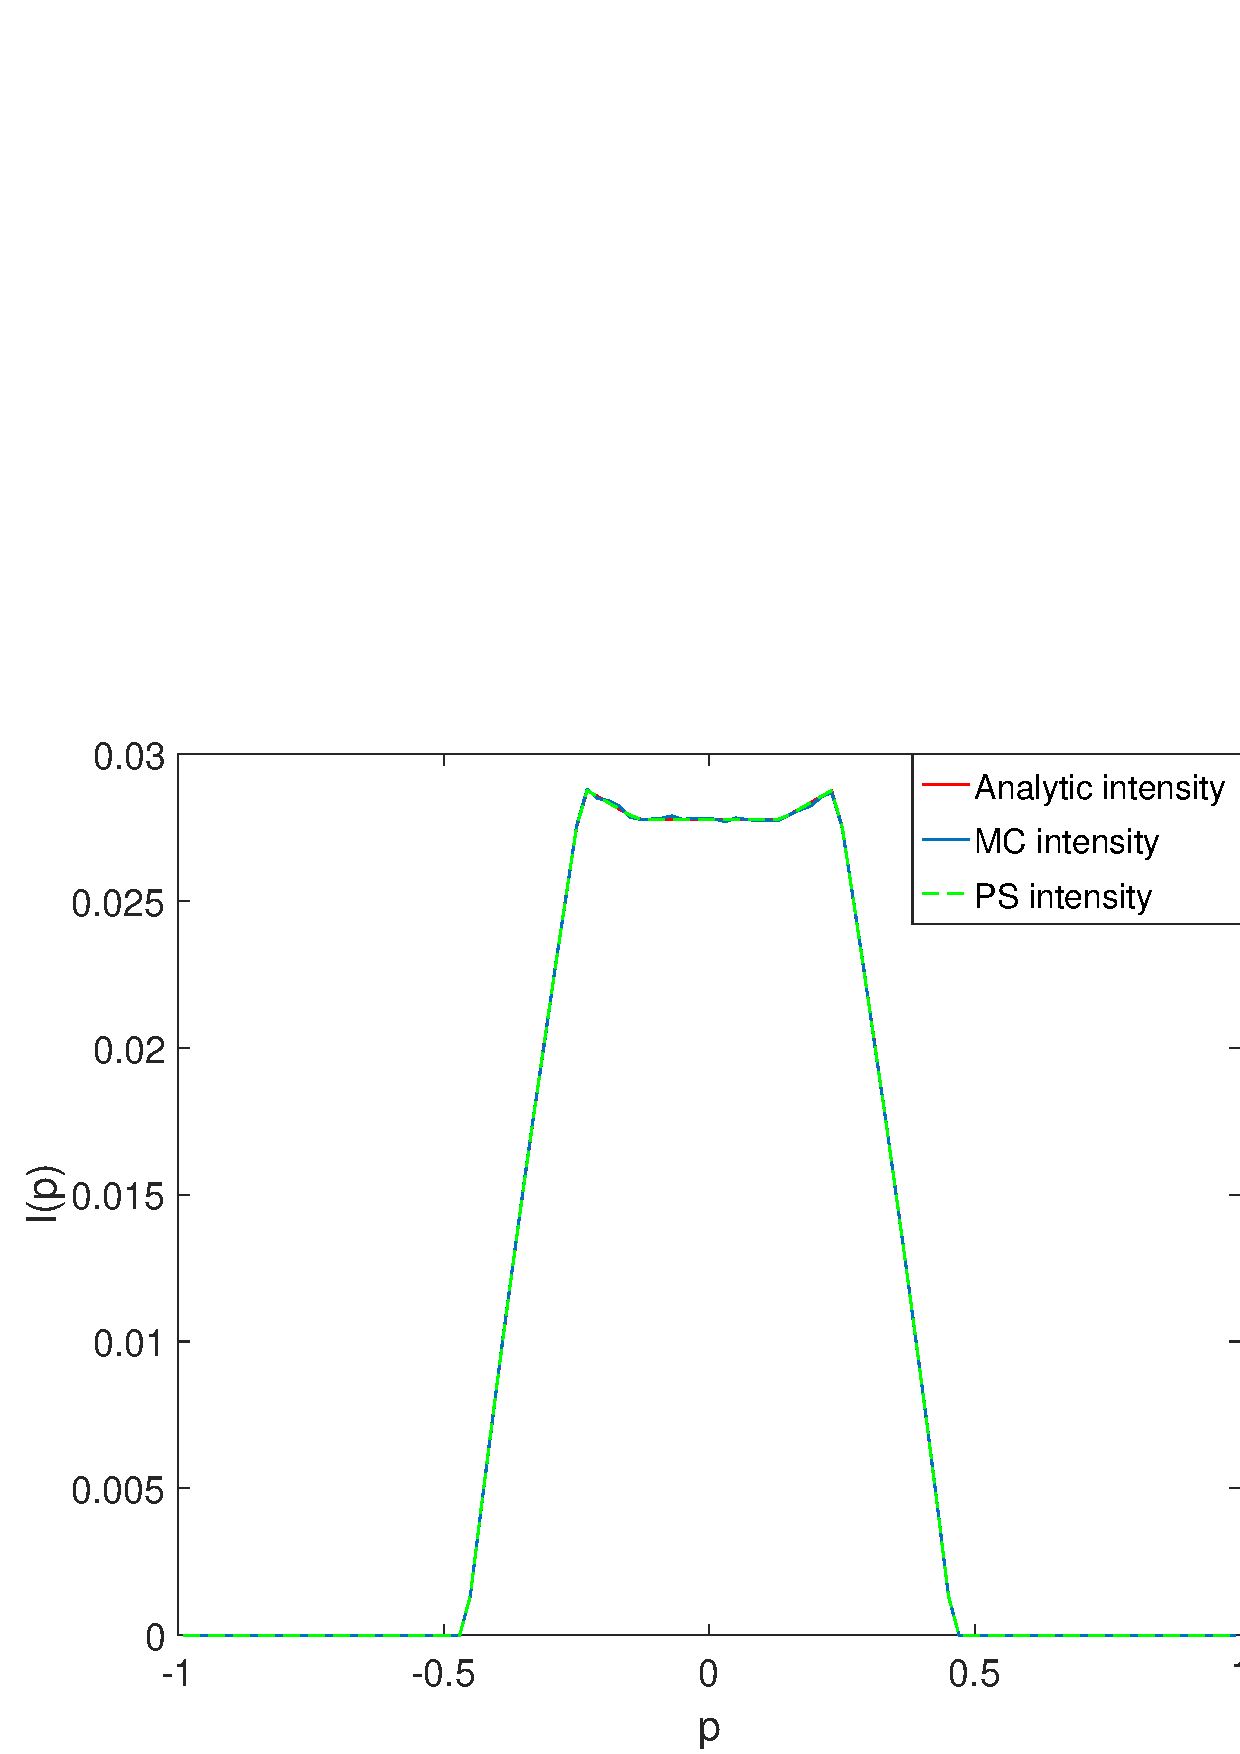
\includegraphics[scale=.4]{intensity.pdf}
%  \end{center}
%  \caption{\footnotesize{Intensities for the two-faceted cup with three different approaches.
%  The red line shows the analytic intensity.
%  The blue line depicts the intensity computed with MC raytracing tracing $10^7$ rays.
%  The dotted green line shows the intensity
%  found with the new method.}}
%  \label{fig:intensity_cup}
%\end{figure}
%\begin{figure}[h]
%  \begin{center}
%  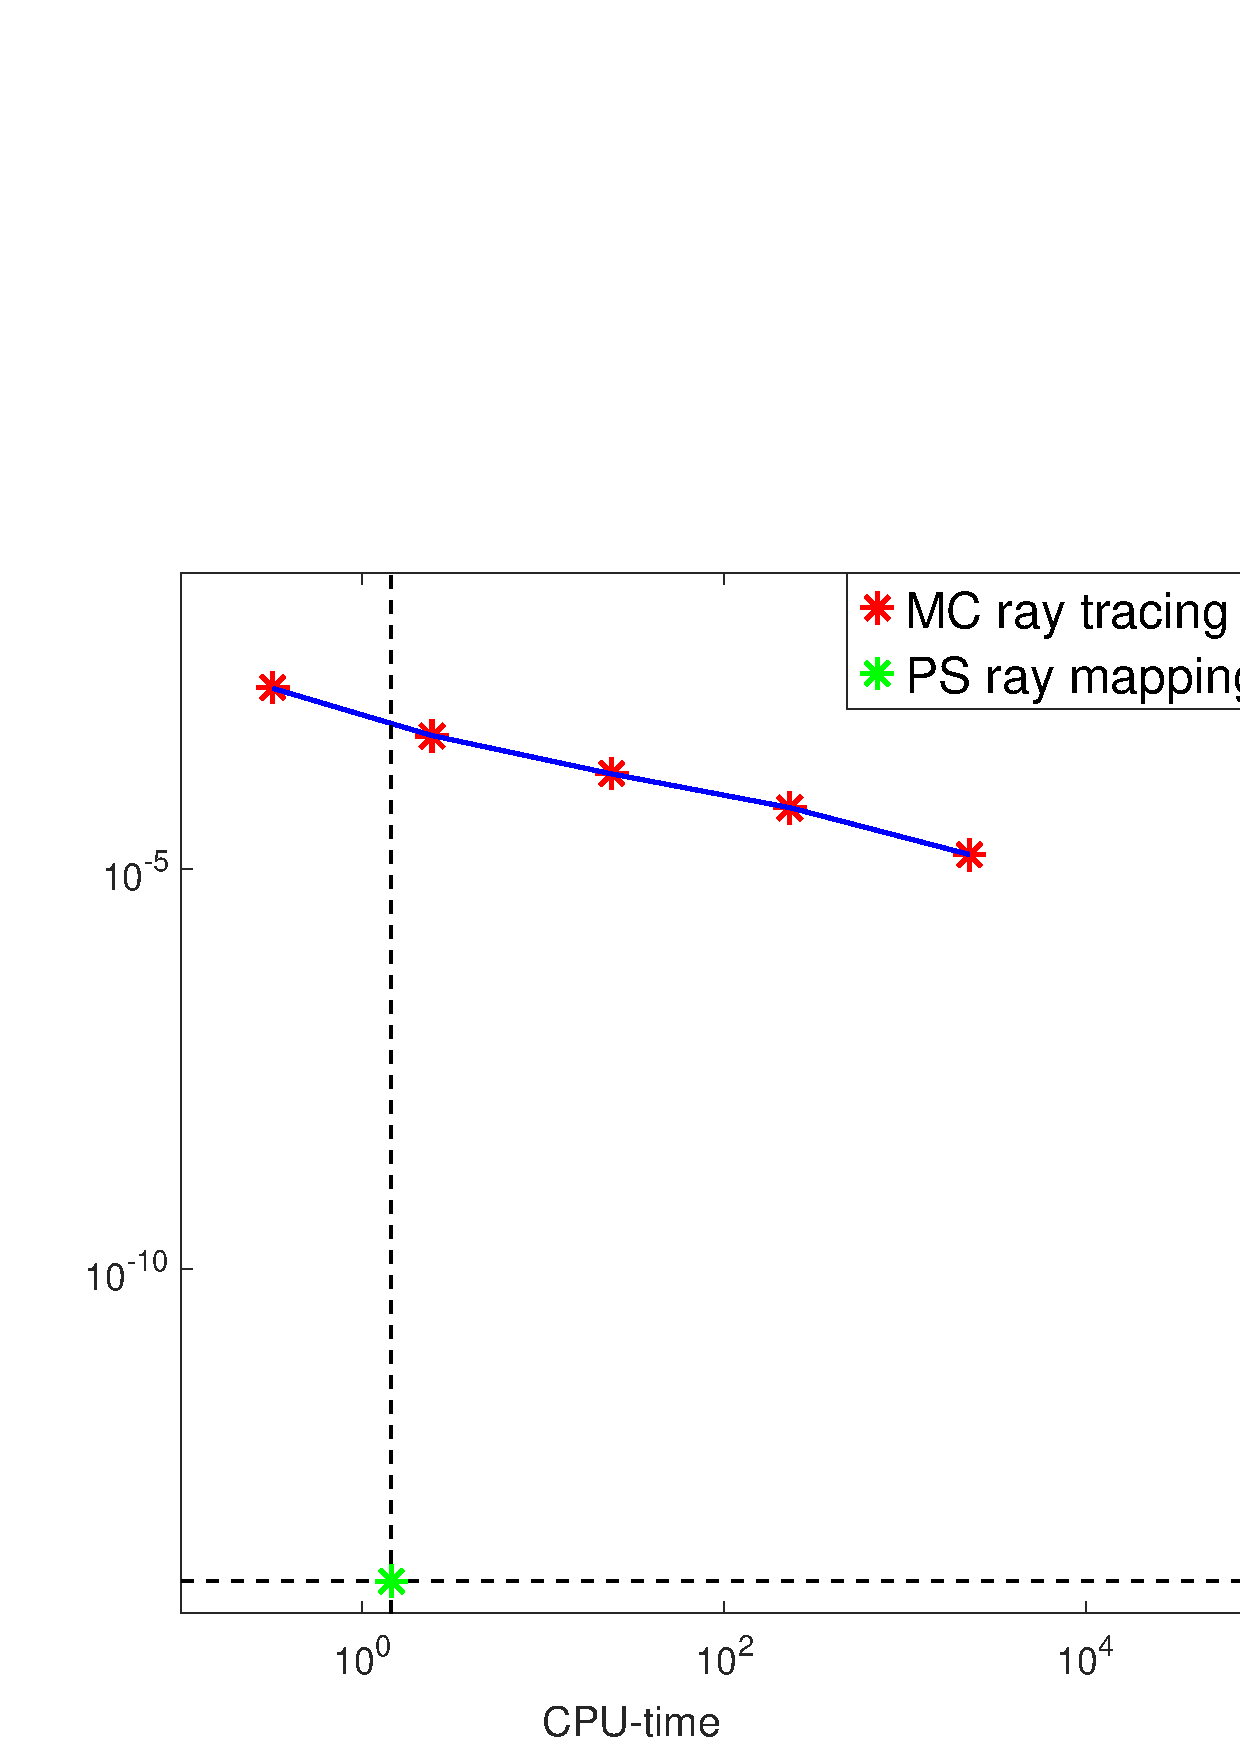
\includegraphics[scale=.5]{error_MC_PS.pdf}
%  \end{center}
%  \caption{\footnotesize{Error between the approximated intensities and the reference intensity as a function of the CPU time.
%  The behavior of the convergence of the ray tracing approach is depicted with the blue line.
%  The error decreases increasing the number of rays traced.
%  The green dot shows the error obtained with the PS method.}}
%  \label{fig:error_cup}
%\end{figure}
%\newpage
%\section{Generalization of the method to other optical systems}
%\label{sec:Generalization}
%The method can be generalized to more complicated optical systems.
%In particular, it can be used for all the systems formed by straight lines.
%The goal of this section is to show the generalization of the method to the multi-faced cup that is a system with many left and right segments as reflectors.
%The design of this system is explained below.
%\subsection{\textbf{The multi-faceted cup}}
%A multi-faceted cup is an optical system formed by a source, a target and $\variable{n}$ left and right reflectors.
%Defining a Cartesian coordinate system $(\variable{x}, \variable{z})$, the multi-faceted cup is symmetric with respect to the optical axis (\variable{z}-axis). \\
%An example of this system is depicted in Fig. \ref{fig:multifacetedcup} where all the lines are labeled with numbers.
%The source $\point{S}= [-\variable{a}, \variable{a}]$ (line $1$) and the target $\point{T}= [-\variable{b}, \variable{b}]$ (line $22$) are two segments both perpendicular to the optical axis, with $\variable{a}=2$ and $\variable{b}=17$.
%$\point{S}$ is located at the height $\variable{z}=0$ while $\point{T}$ has a height $\variable{z}=40$.
%Both sides of the system are divided into $10$ segments which connect $\point{S}$ with $\point{T}$.
%The $10$ adjacent segments at the left of the system (lines $2, \cdots, 11$) connect the left extreme of the source with the left extreme of the target.
%Similarly, $10$ adjacent segments at the right of the system (lines $12, \cdots, 21$) connect the right extreme of the source with the right extreme of the target.
%These segments are designed as follow. The intervals $[-\variable{b}, -\variable{a}]$ and $[\variable{b}, \variable{a}]$ are divided into $10$ bins of the same length $(\variable{b}-\variable{a})/10$.
%The \variable{x}-coordinates of the extremes of the segments (lines $2, \cdots, 21$) are equal to the \variable{x}-coordinates of the bins.
%Therefore, the \variable{x}-coordinates of the extremes of the right segment adjacent to the source (line $2$) are $\variable{a}$ and $\variable{a}+(\variable{b}-\variable{a})/10$;
%the \variable{x}-coordinates of the extremes of the next right segment (line $3$) are $\variable{a}+(\variable{b}-\variable{a})/10$ $\variable{a}+2(\variable{b}-\variable{a})/10$ and so on.
%The \variable{z}-coordinates of every extreme of the intervals are given substituting the $\variable{x}$-coordinates into the equation of the parabola with
%axis equal to the \variable{z}-axis and that passes through the
%points $(-17,40)$ and $(17,40)$. At this point the $20$-faceted cup is well defined and it can be seen as an approximation of a parabolic reflector.
%All the optical lines \variable{i} with $\variable{i} \in \{1, \cdots, 22\}$ are located in air, therefore the refractive index $\variable{n}_{\variable{i}}=1$ for every \variable{i}.
%This system is called the $20$-faceted cup.
%\begin{figure}[h!]
%\centering
%\label{fig:multifacetedcup}
%\includegraphics[scale=.4]{multifacetedcup1.pdf}
%\caption{\footnotesize{Shape of the $20$-faceted cup. The system is formed by $22$ different lines: the source $\point{S}$, the target
%$\point{T}$, $10$ left reflectors and $10$ right reflectors.
% $\point{S}=[-2,2]$ is located at $\variable{z}=0$. $\point{T} = [-17,17]$ is parallel to the source and it is located at a height $\variable{z}=40$.
% The left and the right reflectors are adjacent segments. The \variable{x} coordinates of the extremes of the reflectors are located at the same distance.
% The \variable{z} coordinates are located on a parabola that passes through the extremes of the target and has as symmetric axis the \variable{z}-axis.
% All the lines are located in air.}}
%\label{fig:multifacetedcup} % Give a unique label
%\end{figure}
%Similarly to the two-faceted cup, also for the multi-faceted cup we define the phase spaces of all the lines $\variable{i}\in\{1, \cdots, \variable{n}\}$ as in Section \ref{sec:Phase space}.
%In particular, the source and the target phase spaces are defined for the left and the right reflectors, while only one phase space is defined for the source and one for the target (the source and the target phase space, respectively). For instance, for the system in Figure \ref{fig:multifacetedcup}, $42$ different phase spaces need to be considered.
%In general, for a system formed by $\variable{n}$ straight lines, $2\variable{n}-2$ phase spaces are considered.
%% The phase spaces $\set{S}{i}{}$ and $\set{T}{i}{}$ of each line $\variable{i}=\{1, \cdots, 22\}$ are divided into regions $(\set{S}{i}{,j})_{\variable{j}=2, \cdots, 22}$ and
%% $(\set{T}{i}{,k})_{\variable{k}=1, \codts, 21}$, respectively; where we have used the same notation used in Section \ref{sec:Phase space}
%The phase spaces \set{S}{i}{} and  \set{T}{i}{} of each line \variable{i}$\in \{1, \cdots, \variable{n}\}$ are partitioned into different regions, (\set{S}{i,}{j})$_{\variable{j}=2, \cdots, \variable{n}}$ and (\set{T}{i,}{k})$_{\variable{k}=1, \cdots, \variable{n}-1}$, respectively; where we have used the same notation used in Section \ref{sec:Phase space}.
%The boundaries $(\partial\mbox{\set{S}{i,}{j}})_{\variable{j}=2, \cdots, \variable{n}}$ and $(\partial\mbox{\set{T}{i,}{k}})_{\variable{k}=1, \cdots, \variable{n}-1}$ can be determined analytically as explained in Section \ref{sec:appendix}. \\
%\indent As an example, the boundaries $(\partial\mbox{\set{T}{$22$,}{k}})_{\variable{k}=1, \cdots, 21}$ for the $20$-faceted cup are depicted in Fig. \ref{fig:T20} with red lines.
%The target PS \set{T}{$22$}{} is divided into $21$ different regions, each of them formed by the rays emitted by line $\variable{k}\in\{1, \cdots, 21\}$.
%Note that we always choose the index of the target equal to the index of the number of lines that form the system $\variable{n}$ (indeed, for the $20$-faceted cup, $\variable{n}=22$).
%\begin{figure}[h!]
%\centering
%\label{fig:T20}
%\includegraphics[scale=.4]{target10facetedcup1.pdf}
%\caption{\footnotesize{Target phase space of the $20$-faceted cup.
%The red lines are the boundaries $(\partial\mbox{\set{T}{$22$,}{k}})_{\variable{k}=1, \cdots, 21}$ of the regions $(\mbox{\set{T}{$22$,}{k}})_{\variable{k}=1, \cdots, 21}$
%and they are determined analytically. The numbers inside the regions \set{T}{$22$,}{k} indicate the value of the index \variable{k}.}}
%\label{fig:T20} % Give a unique label
%\end{figure}
%The target intensity $I_{\textrm{PS}}(\variable{p})$ along a given direction $\variable{p}\in [-1, 1]$ in target phase space \set{T}{n,}{} is defined by Eq. (\ref{eq:intensity}).
%Similarly, the target luminance $L(\variable{q}, \variable{p})$ is obtained using
%Eq. (\ref{LT}) with $\variable{n}$, where $\Pi$ is a given path from \point{S} to point \point{T} and \set{R}{}{}$(\Pi)$ is the corresponding region.
%All the possible paths are determined employing the inverse, \inversemap{M}{$1$,}{n}, of the map \map{M}{$1$,}{n}:\set{S}{$1$}{}$\mapsto$\set{T}{n}{}
% which is given by the composition of the propagation and the reflection maps defined in Eqs. (\ref{Pij}) and (\ref{Rj}), respectively.
% As the number of optical lines increases, the number of the possible paths that a ray can follow during its propagation increases as well.
% Therefore, we have to construct a more complicated tree than the one in Fig. \ref{fig:tree} with more vertices corresponding to the same level of the tree.
%Despite this, the algorithm explained in the previous section still works fine and also for the multi-faceted cup we are able to determine all the possible paths and all the regions \set{R}{}{}$(\Pi)$ with positive luminance at target PS \set{T}{n}{}.
%Assuming a Lambertian source, only the rays located at the boundaries of these regions need to be computed.
%Therefore, for a given direction $\variable{p}=\const{const}$ only the coordinates $\variable{q}^\textrm{\,min}(\Pi,\variable{p})$ and $\variable{p}^\textrm{\,max}(\Pi,\variable{p})$ the minimum and maximum position coordinates of the intersection points between the boundaries $ \partial$\set{R}{}{}($\Pi$) and the line $\variable{p}= const$, for every possible path $\Pi$. Finally, the intensity $I_{\textrm{PS}}(\variable{p})$ along the direction $\variable{p}$ is obtained employing Eq. (\ref{eq:intensity}).
%Numerical results for a $20$-faceted cup are given in the next section.
%\section{Numerical results for the generalized system: the $20$-faceted cup}
%\label{sec:Numerical results_10cup}
%In this section the results for the $20$-faceted cup are shown.
%We compute the target intensity both with the ray mapping method and MC ray tracing.
%The two intensities are calculated as explained in Section \ref{sec:Phase space}.
%The same partitioning $P:-1\leq \variable{p}^1 <\cdots <\variable{p}^\textrm{Nb} \leq 1$ of the interval $[-1,1]$ used for the two-faceted cup is considered.
%The number of bins considered is $\textrm{Nb}=100$.
%The normalized MC intensity $\hat{I}_{\textrm{MC}}$ is obtained employing Eq. (\ref{eq:MC_intensity}).
%The normalized PS intensity $ \hat{I}_{\textrm{PS}}$ is computed using Eq. (\ref{eq:intensity}).
%The profile of the intensity is depicted in Fig. \ref{fig:intensity10cup}.
%Both the MC intensity and the PS intensity are shown in that picture.
%They are compared with a reference intensity $\hat{I}_{\textrm{ref}}$ which is found using MC ray tracing and tracing $10^8$ rays.
%\begin{figure}[h!]
%\centering
%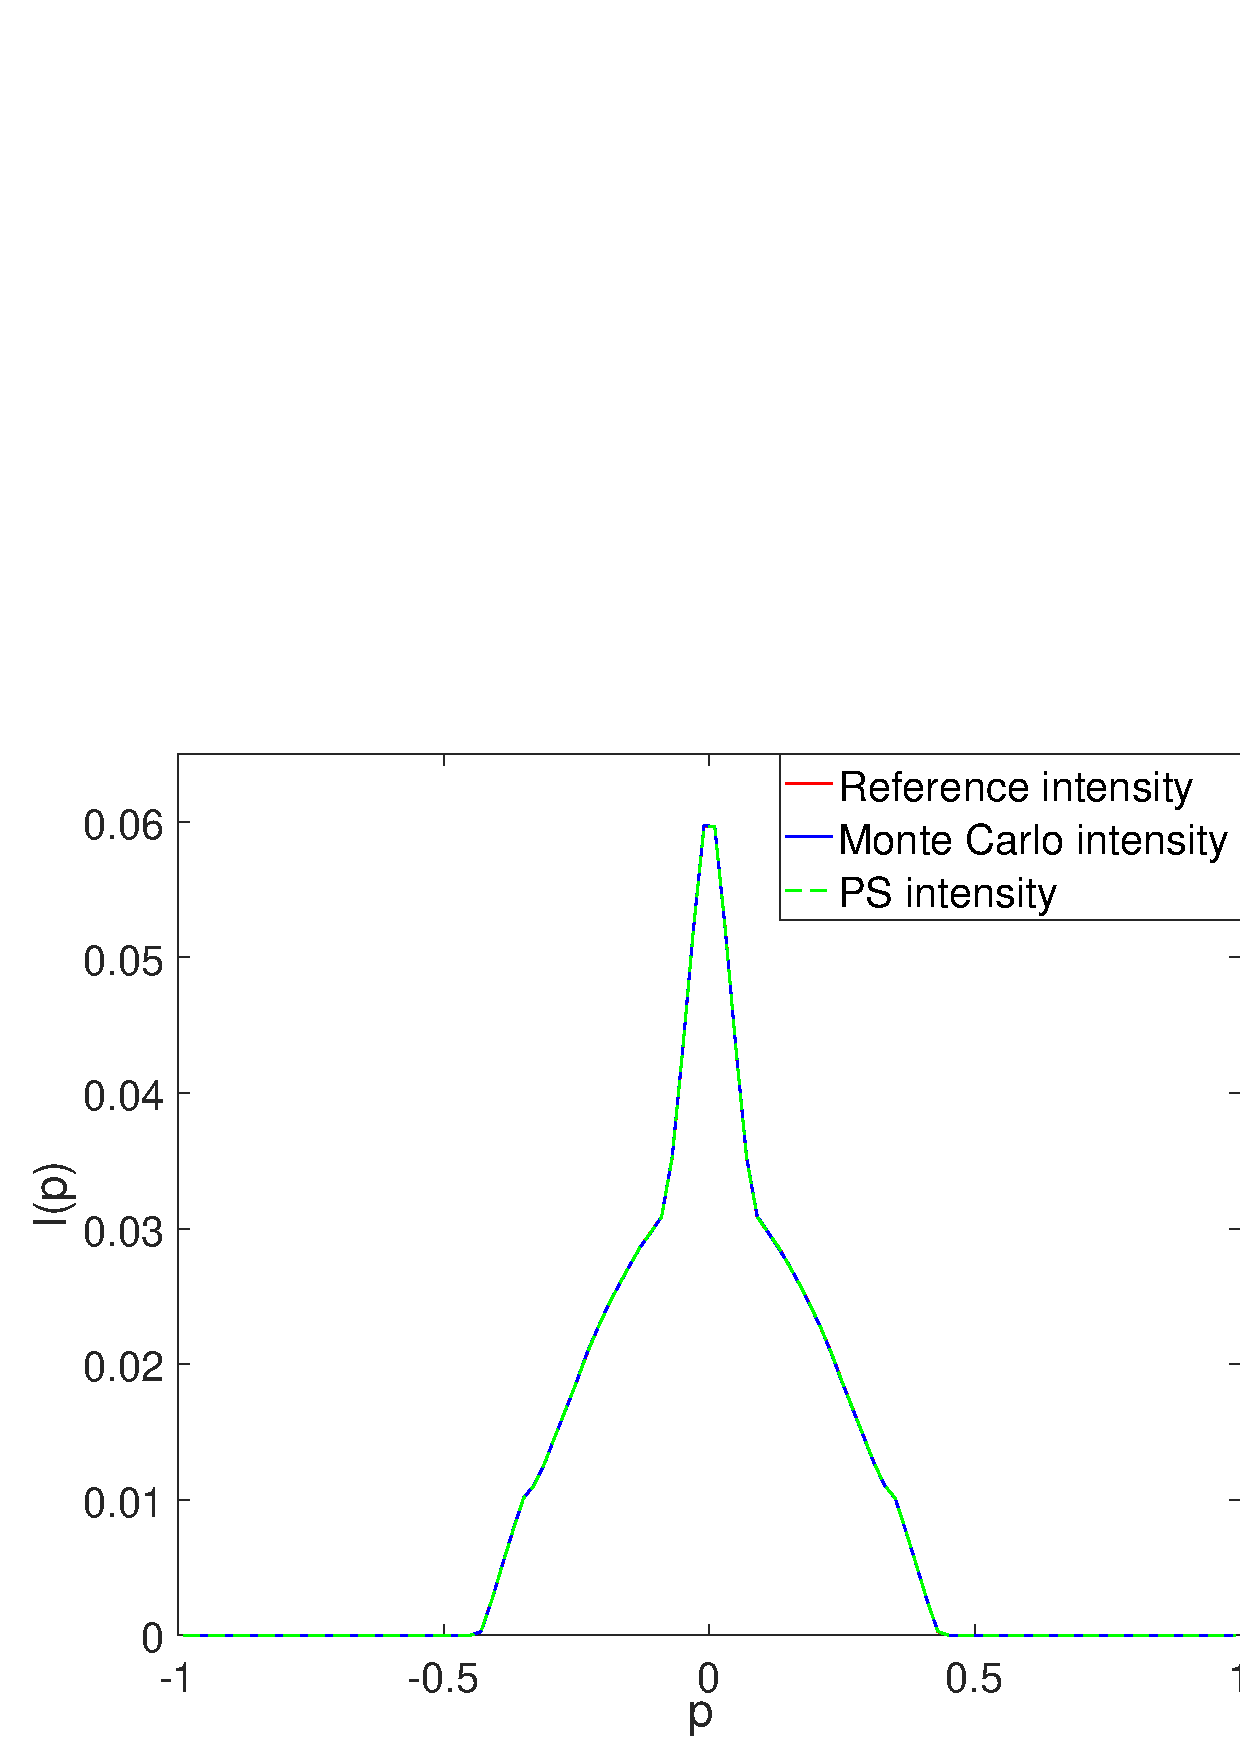
\includegraphics[scale=.4]{intensities10cup.pdf}
%\caption{\footnotesize{Intensity for the $20$-faceted cup.
%The red line shows the reference intensity computed using MC ray tracing and tracing $10^8$ rays.
%The blue line depicts the MC intensity with $10^7$ rays.
%The green and dotted line shows the intensity found with the ray mapping method.}}
%\label{fig:intensity10cup} % Give a unique label
%\end{figure}
%Finally, in order to show the performance of the new method, we calculate the error between the approximate intensities $\hat{I}_{\textrm{A}}$ ($\textrm{A} = \textrm{MC}, \textrm{PS}$) and the reference intensity $\hat{I}_{\textrm{ref}}$ using Eq. (\ref{error}). The MC intensity is calculated
%several times increasing the number of rays traced through the system. Every time, the error between the
%approximate intensity and the reference intensity is calculated using Eq. (16). In Fig. \ref{fig:error10cup} the speed of convergence for MC ray tracing is shown with the blue line. Also, the PS intensity is computed several times increasing every time the number of bins used in the trapezoidal rule to approximate the
%integrals in Eq. (\ref{eq:intensity}). The error for the ray mapping method is calculated for all the approximated intensity.
%Increasing the number of bins in the trapezoidal rule, the PS error decreases. The speed of convergence is depicted in Fig. \ref{error} with the red line.
%Since all the boundaries of the regions in PS are calculated analytically, we expect that the intensity is analytic too.
%From Fig. \ref{fig:error10cup} we observe that the minimum error between the reference intensity and the approximated intensity found with the ray mapping method is equal to
%around $1.87\cdot 10^{-6}$.
%This is due to the fact that we took as reference intensity an intensity computed with MC ray tracing using $7.5*10^8$ rays instead of an analytic intensity.
%In the case of the $20$-faceted cup the reference intensity is not the exact intensity since it suffers of the MC error.
%The error between the exact intensity and $I_{\textrm{exact}}$ the approximate intensity $I_{\textrm{A}}$ is given by:
%\begin{equation}
%\frac{\sum_{\variable{h} = 1}^{\textrm{Nb}}| \hat{I}_{\textrm{exact}}(\variable{p}^\variable{h}) - \hat{I}_{\textrm{A}}(\variable{p}^\variable{h})|}{\textrm{Nb}} \leq
%\frac{1}{\textrm{Nb}}\Bigg(\sum_{\variable{h} = 1}^{\textrm{Nb}}\big| \hat{I}_{\textrm{exact}}(\variable{p}^\variable{h}) - \hat{I}_{\textrm{ref}}(\variable{p}^\variable{h})\big| +
%\sum_{\variable{h} = 1}^{\textrm{Nb}}\big| \hat{I}_{\textrm{ref}}(\variable{p}^\variable{h}) - \hat{I}_{\textrm{A}}(\variable{p}^\variable{h})\big|\Bigg)
%\end{equation}
%Making an extrapolation of MC error we can obtain an approximation of the error between MC ray tracing with $7.5*10^{8}$ rays and the exact intensity,
%this error is depicted in Fig. \ref{fig:error10cup} with the cyan dot.
%Note that $\sum_{\variable{h} = 1}^{\textrm{Nb}}| \hat{I}_{\textrm{exact}}(\variable{p}^\variable{h}) - \hat{I}_{\textrm{ref}}(\variable{p}^\variable{h})|/\textrm{Nb}\approx 1.68*10^{-6}$.
%The results show that $\sum_{\variable{h} = 1}^{\textrm{Nb}}| \hat{I}_{\textrm{exact}}(\variable{p}^\variable{h}) - \hat{I}_{\textrm{ref}}(\variable{p}^\variable{h})|/\textrm{Nb}
%\approx \sum_{\variable{h} = 1}^{\textrm{Nb}}|\hat{I}_{\textrm{ref}}(\variable{p}^\variable{h}) - \hat{I}_{\textrm{PS}}(\variable{p}^\variable{h})|/\textrm{Nb}$.
%Therefore, we can claim that the error found with the inverse ray mapping method is also due to the MC error.
%We can conclude that the inverse ray mapping method performs well also for more complicated systems.
%Compared to MC ray tracing the new method is not only faster but also much more accurate for all the systems formed by straight lines.
%\begin{figure}[h!]
%\centering
%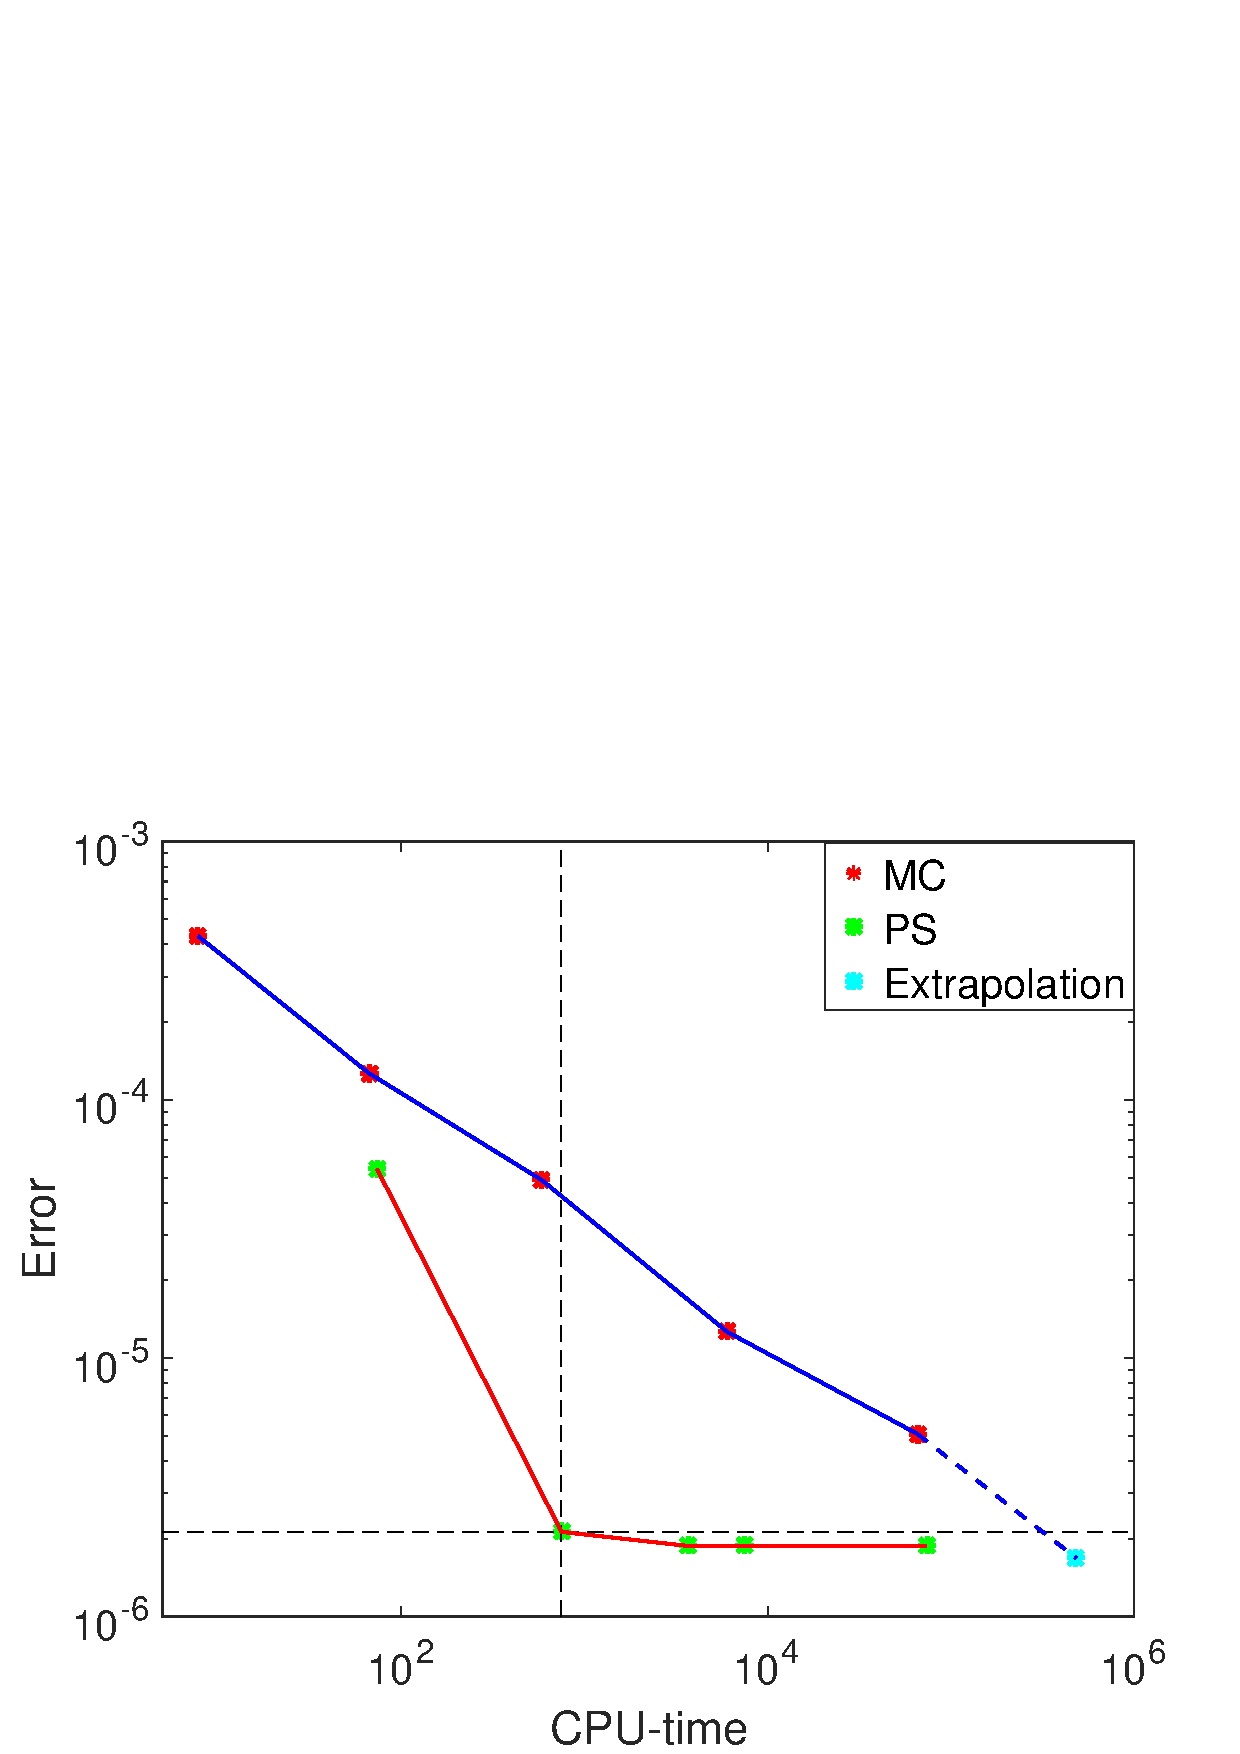
\includegraphics[scale=.4]{error_10cup1.pdf}
%\caption{\footnotesize{Error between the approximated intensities and the reference intensity as a function of the CPU time. The convergence
%of MC ray tracing is depicted with the blue line. The MC error decreases increasing the number of rays traced.
%The green dots show the error obtained with the PS method. The PS error decreases increasing the
%number of bins considered to calculate the integral at the denominator of Eq. (\ref{eq:intensity}). The ray mapping method is more accurate than MC ray tracing and it is faster in case an error smaller than say $10^{-4}$ is desired.}}
%\label{fig:error10cup} % Give a unique label
%\end{figure}
%
%\section{Results for the two-faceted cup}
%\section{Results for the multi-faceted cup}
%\section{Discussions}